% =============================================================
%  BÁO CÁO CUỐI KỲ
%  Môn: An toàn & Bảo mật Hệ thống Thông tin
%  Compile: pdflatex + bibtex  hoặc  xelatex + bibtex
% =============================================================
\documentclass[12pt,a4paper]{report}

% ---- Encoding & ngôn ngữ ----
\usepackage[utf8]{inputenc}
\usepackage[T5]{fontenc}
\usepackage[vietnamese]{babel}

% ---- Layout ----
\usepackage[
  top=3cm, bottom=3cm,
  left=3.5cm, right=2.5cm
]{geometry}
\usepackage{setspace}
\setstretch{1.0}

% ---- Tiêu đề, chương, mục ----
\usepackage{titlesec}
\titleformat{\chapter}[block]
  {\normalfont\large\bfseries\centering}{CHƯƠNG \thechapter.}{0.5em}{}
\titlespacing*{\chapter}{0pt}{0pt}{12pt}
\titlespacing*{\section}{0pt}{8pt}{3pt}
\titlespacing*{\subsection}{0pt}{6pt}{2pt}

% ---- Toán, ký hiệu ----
\usepackage{amsmath,amssymb}
\usepackage{enumitem}
\setlist{itemsep=1pt,topsep=2pt,parsep=0pt,partopsep=0pt}

% ---- Bảng ----
\usepackage{booktabs}
\usepackage{multirow}
\usepackage{array}
\usepackage{longtable}
\usepackage{tabularx}

% ---- Hình ----
\usepackage{graphicx}
\usepackage{float}
\graphicspath{{figures/}}

% ---- Màu, liên kết ----
\usepackage{xcolor}
\usepackage[
  colorlinks=true,
  linkcolor=black,
  citecolor=blue,
  urlcolor=blue
]{hyperref}

% ---- Tài liệu tham khảo ----
\usepackage{cite}

% ---- Placeholder ----
\newcommand{\tbd}[1][TBD]{\textcolor{gray}{\textit{[#1]}}}

% ---- Khoảng cách đoạn ----
\setlength{\parskip}{2pt}
\setlength{\abovecaptionskip}{4pt}
\setlength{\belowcaptionskip}{0pt}
\setlength{\textfloatsep}{8pt}
\setlength{\floatsep}{6pt}
\setlength{\intextsep}{6pt}
\setlength{\parindent}{1.25cm}

% =============================================================
\begin{document}

% =============================================================
%  TRANG BÌA
% =============================================================
\begin{titlepage}
\begin{center}

{\large\bfseries ĐẠI HỌC QUỐC GIA THÀNH PHỐ HỒ CHÍ MINH}\\[4pt]
{\large\bfseries TRƯỜNG ĐẠI HỌC KHOA HỌC TỰ NHIÊN}\\[6pt]
\rule{\textwidth}{1.5pt}\\[6pt]
\rule{\textwidth}{0.5pt}

\vspace{1.5cm}
{\Large\bfseries BÁO CÁO CUỐI KỲ}\\[0.5cm]
{\large Môn học: \textbf{An toàn \& Bảo mật Hệ thống Thông tin}}

\vspace{1.2cm}
\fbox{%
  \parbox{0.92\textwidth}{%
    \vspace{0.4cm}
    \begin{center}
      {\LARGE\bfseries
        Tấn công Suy luận Tư~cách Thành~viên\\[8pt]
        trên các Mô~hình Chuỗi Thời~gian Hiện~đại:\\[8pt]
        Đánh giá hệ thống trên PTB-XL~ECG
      }
    \end{center}
    \vspace{0.4cm}
  }%
}

\vspace{1.2cm}
\begin{minipage}{0.48\textwidth}
\begin{flushleft}
{\large\bfseries Giảng viên hướng dẫn:}\\[4pt]
PGS.TS. Đặng Trần Khánh\\
TS. Phạm Thị Bạch Huệ\\
ThS. Lương Vĩ Minh
\end{flushleft}
\end{minipage}
\hfill
\begin{minipage}{0.48\textwidth}
\begin{flushright}
{\large\bfseries Nhóm thực hiện:}\\[4pt]
25C12008 -- Lê Thành Ngọc\\
25C01025 -- Cao Anh Tuấn\\
25C12018 -- Bùi Lê Hoài An\\
25C12022 -- Trần Trọng Hoàng
\end{flushright}
\end{minipage}

\vfill
{\large TP. Hồ Chí Minh, tháng 10 năm 2026}
\end{center}
\end{titlepage}

% =============================================================
%  TÓM TẮT
% =============================================================
\chapter*{Tóm tắt}
\addcontentsline{toc}{chapter}{Tóm tắt}

Báo cáo này trình bày một nghiên cứu đánh giá hệ thống về \textit{tấn công suy luận tư cách thành viên} (Membership Inference Attack -- MIA) trên các mô hình học sâu xử lý chuỗi thời gian. Đây là một dạng tấn công quyền riêng tư nhằm xác định liệu một bản ghi dữ liệu cụ thể có được sử dụng để huấn luyện mô hình hay không.

Thực nghiệm được tiến hành trên tập dữ liệu ECG công khai PTB-XL với hai bài toán: \textbf{phân loại} (5 lớp chẩn đoán) và \textbf{dự báo} (ngữ cảnh $L = 512$, horizon $H = 96$). Năm mô hình được đánh giá: (1) LSTM và TCN đóng vai trò baseline, (2) PatchTST, (3) iTransformer, và (4) mô hình nền tảng MOMENT được tinh chỉnh toàn bộ trọng số. Sáu họ tấn công (tám cấu hình) được so sánh: Loss, Confidence, Entropy, LiRA (online/offline), RMIA (online/offline) và Temporal Feature.

Kết quả đánh giá theo tiêu chuẩn \textit{low-FPR} (TPR tại 0,1\% và 1\% FPR kèm khoảng tin cậy bootstrap 95\%) cho thấy ba phát hiện chính: (i) trên cả năm mô hình, bài toán dự báo rò rỉ nhiều hơn phân loại, với hệ số chênh từ $1{,}7\times$ (TCN) đến $21\times$ (LSTM) và $15\times$ (PatchTST); (ii) MOMENT sau tinh chỉnh toàn bộ là mô hình rò rỉ nhiều nhất ở cả hai bài toán, đặc biệt trên dự báo, song chênh lệch này đan xen với kích thước mô hình và generalization gap nên không thể quy riêng cho việc tinh chỉnh; (iii) ở phân loại, các tấn công điểm số đơn giản (Loss, Confidence, Entropy) gần như tương đương bộ phân loại ngẫu nhiên tại 0,1\% FPR, trong khi các tấn công dựa trên tỉ lệ khả năng (LiRA, RMIA) hoặc đặc trưng thời gian (Temporal) phát hiện được rò rỉ; riêng iTransformer, chỉ Temporal Feature hiệu quả.

\textbf{Kết quả nổi bật:} MOMENT tinh chỉnh toàn bộ đạt TPR = 97,7\% tại 0,1\% FPR trên bài toán dự báo (AUC = 0,9999), so với chỉ 9,9\% trên phân loại, cho thấy nguy cơ rò rỉ nghiêm trọng khi triển khai foundation model trên dữ liệu y tế nhạy cảm.

% =============================================================
%  MỤC LỤC
% =============================================================
\tableofcontents
\listoftables
\listoffigures

% =============================================================
%  DANH MỤC TỪ VIẾT TẮT
% =============================================================
\chapter*{Danh mục từ viết tắt}
\addcontentsline{toc}{chapter}{Danh mục từ viết tắt}

\begin{tabular}{lp{10cm}}
\textbf{MIA}     & Membership Inference Attack (Tấn công suy luận tư cách thành viên) \\
\textbf{LiRA}    & Likelihood Ratio Attack \\
\textbf{RMIA}    & Reference-based Membership Inference Attack \\
\textbf{TPR}     & True Positive Rate (Tỉ lệ dương tính thật) \\
\textbf{FPR}     & False Positive Rate (Tỉ lệ dương tính giả) \\
\textbf{AUC}     & Area Under the ROC Curve \\
\textbf{ECG}     & Electrocardiogram (Điện tâm đồ) \\
\textbf{LSTM}    & Long Short-Term Memory \\
\textbf{TCN}     & Temporal Convolutional Network \\
\textbf{DFT}     & Discrete Fourier Transform (Biến đổi Fourier rời rạc) \\
\textbf{cls}     & Classification (Phân loại) \\
\textbf{fcst}    & Forecasting (Dự báo) \\
\textbf{CI}      & Confidence Interval (Khoảng tin cậy) \\
\end{tabular}

% =============================================================
%  CHƯƠNG 1 – GIỚI THIỆU
% =============================================================
\chapter{Giới thiệu}

\section{Đặt vấn đề}

Trong những năm gần đây, các mô hình học sâu xử lý chuỗi thời gian đã đạt được độ chính xác cao trong nhiều lĩnh vực quan trọng: chẩn đoán tim mạch từ điện tâm đồ (ECG), phát hiện hoạt động người dùng, dự báo nhu cầu năng lượng, và phân tích dữ liệu tài chính. Song song với sự phát triển đó, mô hình nền tảng (\textit{foundation model}) như MOMENT \cite{goswami2024} -- được huấn luyện trên lượng dữ liệu khổng lồ và tinh chỉnh trên các tác vụ cụ thể -- đang ngày càng được ứng dụng rộng rãi.

Tuy nhiên, việc huấn luyện trên dữ liệu nhạy cảm đặt ra câu hỏi bảo mật cấp bách: \textbf{liệu dữ liệu cá nhân có bị rò rỉ thông qua mô hình không?} Một kẻ tấn công chỉ cần truy cập hộp đen (gửi đầu vào, nhận đầu ra) có thể xác định được liệu hồ sơ ECG của một bệnh nhân cụ thể đã được dùng để huấn luyện hay không -- đây là dạng tấn công gọi là \textit{tấn công suy luận tư cách thành viên} (Membership Inference Attack, MIA) \cite{shokri2017}.

Trong bối cảnh y tế, việc biết một bản ghi ECG có nằm trong tập huấn luyện của một mô hình gắn với một bệnh cụ thể có thể tiết lộ thông tin sức khỏe của bệnh nhân đó, vi phạm quyền riêng tư nghiêm trọng và có thể vi phạm các quy định bảo vệ dữ liệu cá nhân (GDPR, HIPAA).

\section{Khoảng trống nghiên cứu}

Mặc dù MIA đã được nghiên cứu sâu trên dữ liệu ảnh và bảng biểu, miền chuỗi thời gian còn ít được quan tâm. Nhóm xác định hai khoảng trống cụ thể:

\begin{itemize}
  \item \textbf{G1.} Chưa có đánh giá hệ thống MIA trên các kiến trúc chuỗi thời gian hiện đại (PatchTST, iTransformer) và foundation model (MOMENT).
  \item \textbf{G2.} Chưa có so sánh bài toán phân loại và dự báo trên \textit{cùng} tập dữ liệu theo tiêu chuẩn \textit{low-FPR} do Carlini et al.\ \cite{carlini2022} đề xuất.
\end{itemize}

\section{Câu hỏi nghiên cứu}

Từ hai khoảng trống trên, báo cáo đặt ra hai câu hỏi nghiên cứu:

\begin{description}
  \item[\textbf{RQ1.}] Kiến trúc hiện đại (PatchTST, iTransformer) rò rỉ thông tin thành viên nhiều hay ít hơn so với baseline LSTM/TCN, khi generalization gap tương đương?
  \item[\textbf{RQ2.}] Trên cùng dữ liệu $X$, bài toán phân loại hay dự báo dễ bị tấn công hơn ở chế độ low-FPR?
\end{description}

\section{Đóng góp}

Báo cáo này đóng góp:
\begin{enumerate}
  \item Một protocol thực nghiệm chuẩn hóa: phân chia record-level với 8.136 member và 7.636 non-member, bootstrap CI 95\%, seed cố định (= 42), áp dụng nhất quán cho tất cả mô hình.
  \item Kết quả MIA đầy đủ cho cả năm mô hình (LSTM, TCN, PatchTST, iTransformer, MOMENT) trên cả hai bài toán, kèm đối chiếu số liệu với tệp kết quả và mã nguồn.
  \item Phân tích định lượng về khoảng cách rò rỉ giữa hai bài toán (RQ2).
  \item Phân tích các hiện tượng làm sai lệch cách đọc TPR (điểm số bị bão hòa/trùng nhau, tấn công suy biến) và các hạn chế của thiết kế thực nghiệm (Mục~\ref{sec:limitations}).
\end{enumerate}

\section{Cấu trúc báo cáo}

Phần còn lại được tổ chức như sau: Chương~\ref{chap:lythuyet} trình bày cơ sở lý thuyết và các công trình liên quan. Chương~\ref{chap:dataset} mô tả tập dữ liệu và thiết lập thực nghiệm. Chương~\ref{chap:models} giới thiệu các mô hình được đánh giá. Chương~\ref{chap:attacks} trình bày các phương pháp tấn công. Chương~\ref{chap:results} báo cáo kết quả thực nghiệm. Chương~\ref{chap:thaoluan} thảo luận và Chương~\ref{chap:ketluan} kết luận.

% =============================================================
%  CHƯƠNG 2 – CƠ SỞ LÝ THUYẾT
% =============================================================
\chapter{Cơ sở lý thuyết và Tổng quan tài liệu}
\label{chap:lythuyet}

\section{Tấn công suy luận tư cách thành viên}

\subsection{Định nghĩa}

Cho một mô hình $f_\theta$ được huấn luyện trên tập $D_{train}$ và một bản ghi $(x, y)$, tấn công suy luận tư cách thành viên (MIA) tìm hàm $\mathcal{A}$ sao cho:
\[
  \mathcal{A}(x, y, f_\theta) \in \{\text{member}, \text{non-member}\}
\]
với \textit{member} nghĩa là $(x, y) \in D_{train}$.

\subsection{Tấn công shadow training (Shokri et al., 2017)}

Shokri et al.\ \cite{shokri2017} đề xuất phương pháp \textit{shadow training}: huấn luyện $K$ mô hình bóng (shadow models) bắt chước hành vi của mô hình đích nhưng biết rõ nhãn thành viên, từ đó huấn luyện attack model phân loại member/non-member. Đây là framework nền tảng của các tấn công hiện đại.

\subsection{Tấn công dựa trên điểm số đơn giản}

Song và Mittal \cite{song2021} đánh giá hệ thống ba tấn công đơn giản hơn, không cần shadow model:
\begin{itemize}
  \item \textbf{Loss}: Sử dụng trực tiếp cross-entropy loss làm điểm thành viên (loss thấp $\Rightarrow$ khả năng cao là member).
  \item \textbf{Confidence}: Sử dụng xác suất dự đoán lớn nhất làm điểm thành viên.
  \item \textbf{Entropy}: Sử dụng âm entropy Shannon của phân phối đầu ra.
\end{itemize}
Yeom et al.\ \cite{yeom2018} chứng minh về mặt lý thuyết rằng khoảng cách tổng quát hóa (generalization gap) là điều kiện cần thiết để các tấn công Loss hoạt động.

\subsection{Calibration theo độ khó (Watson et al., 2022)}

Watson et al.\ \cite{watson2022} đề xuất hiệu chỉnh điểm thành viên theo \textit{độ khó} của mẫu: thay vì so sánh loss tuyệt đối, chuẩn hóa loss của mô hình đích với loss kỳ vọng dưới phân phối dữ liệu. Cách tiếp cận này giảm nhiễu do độ biến động tự nhiên của dữ liệu.

\subsection{LiRA -- Likelihood Ratio Attack (Carlini et al., 2022)}

Carlini et al.\ \cite{carlini2022} đề xuất LiRA, tấn công tiên tiến nhất hiện nay:
\begin{enumerate}
  \item Huấn luyện $K$ \textit{shadow models} -- một nửa với bản ghi mục tiêu (IN), nửa còn lại không (OUT).
  \item Với mỗi shadow model, ghi nhận điểm $\phi(x)$ (trong cài đặt của nhóm: $\phi = \log\frac{p}{1-p}$ với $p$ là xác suất của nhãn đúng khi phân loại, và $\phi = -\log \mathrm{MSE}$ khi dự báo).
  \item Ước lượng $\mu_{in}, \mu_{out}$ theo từng bản ghi và độ lệch chuẩn $\sigma_{in}, \sigma_{out}$ \textit{dùng chung toàn cục} (global variance) -- cách làm của nhóm, vì mỗi bản ghi chỉ có $K/2 = 4$ quan sát IN và 4 quan sát OUT.
  \item Điểm tấn công = log-likelihood ratio: $\Lambda(x) = \log \mathcal{N}(\phi(x); \mu_{in}, \sigma_{in}^2) - \log \mathcal{N}(\phi(x); \mu_{out}, \sigma_{out}^2)$.
\end{enumerate}
LiRA có hai biến thể: \textbf{online} (dùng cả quan sát IN lẫn OUT của mỗi bản ghi; yêu cầu kẻ tấn công biết trước bản ghi mục tiêu để đưa vào tập huấn luyện shadow) và \textbf{offline} (chỉ dùng phân phối OUT, điểm tấn công là z-score $(\phi(x) - \mu_{out})/\sigma_{out}$).

Bài báo cũng đề xuất tiêu chuẩn đánh giá \textit{low-FPR}: báo cáo TPR tại FPR = 0,1\% và 1\% thay vì chỉ dùng AUC, vì AUC có thể bị chi phối bởi vùng high-FPR không có ý nghĩa thực tế.

\subsection{RMIA -- Reference-based MIA (Zarifzadeh et al., 2024)}

Zarifzadeh et al.\ \cite{zarifzadeh2024} đề xuất RMIA, phương pháp sử dụng các \textit{bản ghi tham chiếu} $z$ từ quần thể để xấp xỉ likelihood ratio:
\[
  \Lambda_{RMIA}(x) = \Pr_{z \sim \mathcal{D}}\!\left[\frac{p(x \mid \theta)/\bar{p}(x)}{p(z \mid \theta)/\bar{p}(z)} \ge \gamma\right]
\]
Theo tác giả, RMIA ổn định hơn LiRA khi số shadow model nhỏ ($K = 8$ trong báo cáo này), phù hợp với điều kiện tài nguyên hạn chế.

\subsection{Enhanced MIA (Ye et al., 2022)}

Ye et al.\ \cite{ye2022} xây dựng khung kiểm định giả thuyết (hypothesis testing) cho MIA và đề xuất các tấn công dùng \textit{mô hình tham chiếu} (reference model) để hiệu chỉnh theo độ khó của từng mẫu, đạt TPR cao hơn ở mọi mức FPR. Ý tưởng hiệu chỉnh này là tiền đề trực tiếp của LiRA và RMIA; các tấn công này không đòi hỏi truy cập gradient.

\subsection{MIA trên chuỗi thời gian}

Koren et al.\ \cite{koren2025} là một trong những nghiên cứu đầu tiên về MIA trên mô hình \textit{dự báo} chuỗi thời gian. Họ đề xuất hai nhóm đặc trưng tấn công dựa trên hai thành phần cơ bản của chuỗi thời gian: tính mùa vụ (ước lượng bằng biến đổi Fourier) và xu hướng (xấp xỉ bằng đa thức bậc thấp). Các đặc trưng này giúp cải thiện AUC từ 3\% đến 26\% và tăng TPR ở FPR thấp tới 12 lần so với các tấn công tổng quát. Báo cáo này vận dụng ý tưởng đó trong tấn công \textit{Temporal Feature} (Mục~\ref{sec:temporal}).

Johansson et al.\ \cite{johansson2025} đề xuất LiRA đa biến và tấn công học đầu-cuối DTS cho mô hình dự báo (LSTM, N-HiTS) trên dữ liệu EEG và điện năng, ở cả mức bản ghi lẫn mức người dùng. Họ ghi nhận mô hình dự báo dễ bị tổn thương và mức độ này tăng khi horizon dài hơn hoặc tập huấn luyện nhỏ hơn. Công trình đó không so sánh trực tiếp với phân loại; phép so sánh cùng dữ liệu giữa hai bài toán là đóng góp của báo cáo này (G2).

Duan et al.\ \cite{duan2024} cho thấy trên các mô hình ngôn ngữ lớn được tiền huấn luyện (khoảng một epoch trên tập rất lớn), hầu hết MIA chỉ nhỉnh hơn đoán ngẫu nhiên, trái với các kết quả thành công trước đó trên mô hình tinh chỉnh nhiều epoch. Quan sát này gợi ý rằng mức rò rỉ phụ thuộc mạnh vào số lần mô hình nhìn lại dữ liệu và tỉ lệ dữ liệu/tham số.

\section{Các kiến trúc mô hình chuỗi thời gian}

\subsection{LSTM và TCN -- Baseline}

\textbf{LSTM} (Long Short-Term Memory) \cite{hochreiter1997} là kiến trúc hồi tiếp cổ điển với ba cổng (forget, input, output) kiểm soát luồng thông tin qua thời gian. Mỗi bước thời gian, LSTM cập nhật trạng thái ẩn $h_t$ và trạng thái tế bào $c_t$:
\[
  c_t = f_t \odot c_{t-1} + i_t \odot \tilde{c}_t, \quad h_t = o_t \odot \tanh(c_t)
\]
Nhờ cơ chế cổng, LSTM có thể ghi nhớ phụ thuộc dài hạn mà RNN truyền thống không xử lý được.

\textbf{TCN} (Temporal Convolutional Network) \cite{bai2018tcn} thay thế hồi tiếp bằng tích chập nhân quả có dilated, giúp nắm bắt phụ thuộc tầm xa với chi phí song song hóa cao hơn LSTM. Với dilation $d$ và kernel size $k$, trường tiếp nhận (receptive field) của $n$ khối (mỗi khối gồm hai tích chập) là $1 + 2(k-1)\sum_{i=0}^{n-1} 2^i = 1 + 2(k-1)(2^n-1)$. TCN còn sử dụng kết nối tắt (residual) để ổn định huấn luyện.

Cả hai đóng vai trò \textbf{baseline} để đối chiếu với các kiến trúc hiện đại.

\subsection{PatchTST (Nie et al., 2023)}

PatchTST \cite{nie2023} áp dụng ý tưởng patching của Vision Transformer cho chuỗi thời gian bằng cách phân đoạn tín hiệu thành các \textit{patch}. Điểm nổi bật:

\begin{itemize}
  \item \textbf{Patching:} Chuỗi $L$ bước được chia thành $N = \lfloor (L-P)/S \rfloor + 1$ patch dài $P$ bước với bước trượt $S$, mỗi patch là một token. Với $L = 512$, $P = 16$, $S = 8$ (cấu hình của nhóm, các patch chồng lấp một nửa): $N = 63$ token/kênh.
  \item \textbf{Channel independence (CI):} Mỗi kênh được xử lý độc lập bởi cùng một Transformer encoder, giảm overfitting trên dữ liệu đa biến.
  \item \textbf{Transformer encoder:} Multi-head self-attention + FFN chuẩn. Các patch token nắm bắt đặc trưng cục bộ (trong patch) và toàn cục (giữa các patch).
  \item \textbf{Phức tạp tính toán:} $O(N^2 \cdot d_{model})$ thay vì $O(L^2 \cdot d_{model})$, giảm đáng kể vì $N \ll L$.
\end{itemize}

\subsection{iTransformer (Liu et al., 2024)}

iTransformer \cite{liu2024} đề xuất một cách nhìn \textit{đảo ngược} về tokenization trong Transformer:

\begin{itemize}
  \item \textbf{Inverted embedding:} Thay vì mỗi token là một bước thời gian (như Transformer chuẩn), mỗi token là \textit{toàn bộ chuỗi thời gian} của một biến (kênh/variate). Với ECG 12 kênh: 12 token đầu vào, mỗi token là chuỗi $L = 512$ điểm được chiếu lên không gian $d_{model}$ chiều.
  \item \textbf{Attention liên biến:} Multi-head attention nắm bắt tương quan giữa các kênh ECG (ví dụ: tương quan I, II, III, aVR, aVL, aVF...) thay vì phụ thuộc thời gian.
  \item \textbf{Feed-forward:} Áp dụng độc lập trên từng token (tức từng kênh), nắm bắt đặc trưng phi tuyến theo thời gian cho từng kênh.
\end{itemize}

Kiến trúc này đặc biệt phù hợp cho ECG 12 kênh vì các kênh có mối tương quan vật lý mạnh (đều đo điện thế tim từ các góc khác nhau).

\subsection{MOMENT -- Foundation Model (Goswami et al., 2024)}

MOMENT \cite{goswami2024} là họ mô hình nền tảng đầu tiên được thiết kế riêng cho chuỗi thời gian:

\begin{itemize}
  \item \textbf{Kiến trúc:} Dựa trên T5 encoder (Transformer thuần encoder), xử lý từng kênh độc lập với patch tokenization (độ dài patch 8 bước, không chồng lấp). Với $L = 512$: 64 patch token/kênh; các biểu diễn được gộp (mean pooling) trước head xuôi dòng.
  \item \textbf{Tham số:} \texttt{MOMENT-1-large} có khoảng 385M tham số.
  \item \textbf{Pre-training:} Huấn luyện trước trên \textit{Time Series Pile} -- tập dữ liệu công khai gồm khoảng 13 triệu chuỗi thời gian thuộc 13 miền (y tế, kỹ thuật, tài chính...). Mục tiêu: masked patch modeling (che 30\% patch rồi tái tạo).
  \item \textbf{Fine-tuning:} Thêm head tuyến tính cho bài toán xuôi dòng; tinh chỉnh toàn bộ trọng số mô hình.
\end{itemize}

Tương tự BERT trong NLP, MOMENT khai thác kiến thức phổ quát từ pre-training và nhanh chóng thích nghi với tác vụ cụ thể với ít dữ liệu hơn.

% =============================================================
%  CHƯƠNG 3 – TẬP DỮ LIỆU VÀ THIẾT LẬP THỰC NGHIỆM
% =============================================================
\chapter{Tập dữ liệu và Thiết lập thực nghiệm}
\label{chap:dataset}

\section{Tập dữ liệu PTB-XL}

\subsection{Mô tả}

PTB-XL \cite{ptbxl} là tập dữ liệu điện tâm đồ (ECG) 12 kênh lớn nhất hiện có dưới giấy phép mở (PhysioNet \cite{physionet}, CC BY 4.0). Tập dữ liệu bao gồm:
\begin{itemize}
  \item 21.837 bản ghi ECG từ 18.869 bệnh nhân.
  \item Mỗi bản ghi dài 10 giây, tần số lấy mẫu 100\,Hz (phiên bản đầy đủ: 500\,Hz).
  \item 12 kênh (lead) tiêu chuẩn: I, II, III, aVR, aVL, aVF, V1--V6.
  \item Nhãn SCP phân cấp: siêu lớp chẩn đoán, lớp con, và cường độ.
  \item Trường \texttt{patient\_id} để nhận dạng bệnh nhân.
\end{itemize}
Báo cáo chỉ dùng các bản ghi có \textit{đúng một} siêu lớp chẩn đoán: \textbf{16.272 bản ghi từ 14.641 bệnh nhân} (phần còn lại có nhiều hoặc không có siêu lớp nên bị loại).

\subsection{Tiền xử lý}

Mỗi bản ghi được nội suy tuyến tính từ 1.000 điểm (10 giây $\times$ 100\,Hz) về chuỗi $L + H = 608$ điểm, chuẩn hóa z-score theo từng kênh trên từng bản ghi (cùng một cách cho member và non-member), không dùng augmentation, sau đó:
\begin{itemize}
  \item \textbf{Bài toán phân loại}: cắt $L = 512$ điểm đầu làm đầu vào.
  \item \textbf{Bài toán dự báo}: sử dụng 512 điểm đầu làm ngữ cảnh, 96 điểm tiếp theo ($H = 96$) làm nhãn đầu ra.
\end{itemize}
Đầu vào có dạng tensor $12 \times 512$ (12 kênh, 512 bước thời gian). Lưu ý: vì z-score tính trên cả cửa sổ $L + H$, thống kê chuẩn hóa của bài toán dự báo có chứa thông tin của đoạn mục tiêu; điều này áp dụng đồng nhất cho member và non-member nên không tạo chênh lệch giữa hai nhóm.

\subsection{Nhãn phân loại}

Nhóm sử dụng 5 siêu lớp chẩn đoán của PTB-XL: \textbf{NORM} (bình thường), \textbf{MI} (nhồi máu cơ tim), \textbf{STTC} (thay đổi ST/T), \textbf{CD} (rối loạn dẫn truyền), \textbf{HYP} (phì đại). Lớp NORM chiếm khoảng 56\% (4.542/8.136 bản ghi member) nên accuracy cần được đọc cùng tỉ lệ lớp đa số.

\section{Phân chia dữ liệu và Protocol thực nghiệm}

\subsection{Phân chia record-level}

Nhóm áp dụng phân chia \textbf{record-level có phân tầng} (stratified theo siêu lớp): 16.272 bản ghi được chia 50/50 thành \textit{member} (8.136) và \textit{non-member}; từ non-member tách 500 bản ghi làm tập \textit{val} (chỉ dùng để chọn siêu tham số theo utility, không dùng cho tấn công), còn 7.636 bản ghi là non-member dùng để đánh giá. Hệ quả:
\begin{itemize}
  \item Vì chia ở mức bản ghi (không phải bệnh nhân), một bệnh nhân có thể có bản ghi ở cả hai tập: theo \texttt{meta.json}, member có 7.696 bệnh nhân và non-member (test) có 7.211, trong khi tổng chỉ là 14.641, nên có \textit{ít nhất} 266 bệnh nhân xuất hiện ở cả hai phía. Đây là thiết lập record-level theo đúng định nghĩa MIA mức bản ghi, nhưng không phải mức người dùng.
  \item Tỉ lệ lớp trong mỗi tập gần như nhau (stratified by superclass).
  \item Số non-member là 7.636, thấp hơn mục tiêu 10.000 đặt ra ban đầu: tại FPR $= 0{,}1\%$ chỉ cho phép khoảng $7$ non-member bị nhận nhầm, nên TPR@0,1\% FPR có độ phân giải thô và khoảng tin cậy rộng (xem Mục~\ref{sec:limitations}).
\end{itemize}

Phân chia được cố định bởi \textbf{seed = 42} và lưu tại \texttt{dataset/splits/} (kèm mã băm SHA-256 được kiểm tra trước mỗi lần chạy) để đảm bảo tái hiện kết quả trên tất cả mô hình.

\begin{table}[H]
\centering
\caption{Thống kê phân chia dữ liệu (seed = 42; tổng 16.272 bản ghi)}
\label{tab:split}
\begin{tabular}{lcc}
\toprule
\textbf{Tập} & \textbf{Số bản ghi} & \textbf{Vai trò} \\
\midrule
Member (tập huấn luyện)     & 8.136  & Huấn luyện mô hình đích \\
Non-member (tập kiểm tra)   & 7.636  & Dữ liệu không được huấn luyện \\
Validation (từ non-member)  & 500    & Chọn siêu tham số, không dùng để tấn công \\
\midrule
Tổng dùng để đánh giá MIA   & 15.772 & member + non-member \\
\bottomrule
\end{tabular}
\end{table}

\subsection{Shadow models}

Với các tấn công cần shadow model (LiRA, RMIA), nhóm huấn luyện $K = 8$ shadow model theo mặt nạ cố định \texttt{shadow\_masks\_record\_K8\_s42.npz}: mỗi shadow được huấn luyện trên một nửa \textit{toàn bộ} 16.272 bản ghi (gồm cả member lẫn non-member của mô hình đích) và mỗi bản ghi nằm trong đúng 4 shadow (IN) và vắng mặt ở 4 shadow còn lại (OUT). Mỗi shadow dùng \textit{đúng công thức huấn luyện cuối cùng của mô hình đích} (số epoch, learning rate, kiến trúc), chỉ khác tập huấn luyện. Tập tham chiếu của RMIA gồm 5.000 bản ghi lấy từ cùng mặt nạ.

\section{Mô hình đe dọa (Threat Model)}

\textbf{Kẻ tấn công hộp đen (black-box):} Kẻ tấn công chỉ có quyền truy vấn mô hình đích -- gửi đầu vào $x$ và nhận đầu ra $f(x)$ (phân phối xác suất với bài toán phân loại; chuỗi dự báo với bài toán dự báo). Kẻ tấn công không biết trọng số, kiến trúc, hay siêu tham số của mô hình.

Với các tấn công shadow (LiRA, RMIA), kẻ tấn công giả định biết phân phối dữ liệu $\mathcal{D}$ và sở hữu một tập bản ghi gồm cả mẫu mục tiêu để huấn luyện shadow model. Biến thể \textit{online} mạnh hơn \textit{offline} ở chỗ kẻ tấn công còn biết các bản ghi mục tiêu để đưa vào nhóm IN; do đó kết quả online nên được đọc như cận trên về khả năng của kẻ tấn công.

\textbf{Tấn công Temporal Feature} hoạt động ở chế độ \textbf{gray-box}: kẻ tấn công có thêm (i) một tập con có nhãn member/non-member để huấn luyện bộ phân loại (đánh giá bằng cross-fitting 5-fold sao cho mỗi bản ghi được chấm bởi bộ phân loại chưa thấy nó), và (ii) với bài toán phân loại, các checkpoint trung gian của mô hình đích. Đây là giả định mạnh hơn so với black-box thuần túy, nên điểm số Temporal không so sánh ngang hàng được với Loss/LiRA.

\section{Tiêu chuẩn đánh giá}

Theo khuyến nghị của Carlini et al.\ \cite{carlini2022}, nhóm báo cáo:

\begin{itemize}
  \item \textbf{TPR @ 0,1\% FPR}: Tỉ lệ phát hiện đúng member khi chỉ cho phép 0,1\% phát hiện nhầm non-member. Đây là \textit{chỉ số chính}.
  \item \textbf{TPR @ 1\% FPR}: Chỉ số phụ mở rộng vùng low-FPR.
  \item \textbf{AUC}: Diện tích dưới đường ROC. Chỉ dùng để đối chiếu, không phải chỉ số chính.
  \item \textbf{Khoảng tin cậy bootstrap 95\%}: 1.000 lần lấy mẫu lại, member và non-member được lấy mẫu \textit{độc lập}. TPR tại một ngưỡng FPR được lấy là giá trị TPR lớn nhất trong số các ngưỡng có FPR không vượt quá mức đó.
\end{itemize}

\textbf{Lý do chọn low-FPR:} Trong bối cảnh thực tế, kẻ tấn công cần xác định đúng membership với ít sai lầm. AUC cao có thể đến từ vùng high-FPR không có giá trị thực tiễn; TPR @ 0,1\% FPR đo lường chính xác khả năng tấn công có độ tin cậy cao.

% =============================================================
%  CHƯƠNG 4 – CÁC MÔ HÌNH
% =============================================================
\chapter{Các mô hình học sâu được đánh giá}
\label{chap:models}

\section{Phân công và cấu hình chung}

Mỗi thành viên nhóm chịu trách nhiệm toàn bộ pipeline (huấn luyện, tấn công, phân tích) cho một họ mô hình. Bảng~\ref{tab:phancon} tóm tắt phân công.

\begin{table}[H]
\centering
\caption{Phân công thành viên nhóm}
\label{tab:phancon}
\begin{tabular}{clll}
\toprule
\textbf{TV} & \textbf{Họ tên} & \textbf{Mô hình} & \textbf{MSSV} \\
\midrule
TV1 & Bùi Lê Hoài An   & LSTM, TCN (baseline)       & 25C12018 \\
TV2 & Trần Trọng Hoàng & PatchTST                   & 25C12022 \\
TV3 & Cao Anh Tuấn     & iTransformer               & 25C01025 \\
TV4 & Lê Thành Ngọc    & MOMENT (foundation model)  & 25C12008 \\
\bottomrule
\end{tabular}
\end{table}

Tất cả mô hình dùng chung: tập dữ liệu PTB-XL, phân chia record-level cố định (seed = 42), và bộ đánh giá MIA thống nhất (TPR@FPR, bootstrap CI).

\section{LSTM và TCN -- Baseline (TV1: Bùi Lê Hoài An)}

\subsection{LSTM}

LSTM hai lớp một chiều, kích thước ẩn 128, dropout 0,1; đầu vào là chuỗi 12 kênh, lấy trạng thái ẩn ở bước cuối đưa vào một lớp tuyến tính:
\begin{itemize}
  \item Phân loại: head $128 \to 5$, hàm mất mát cross-entropy.
  \item Dự báo: head $128 \to H \times 12$, hàm mất mát MSE.
\end{itemize}
Công thức huấn luyện: AdamW, OneCycleLR, batch 16, gradient clipping 1,0 (xem Bảng~\ref{tab:hparams}).

\subsection{TCN}

TCN với tích chập nhân quả có dilated \cite{bai2018tcn}, cấu hình:
\begin{itemize}
  \item 7 khối tích chập (mỗi khối hai tích chập có weight norm, ReLU, dropout 0,1), kernel $k = 5$, dilation $d = 2^i$, $i = 0, \ldots, 6$; 64 kênh mỗi khối, kết nối tắt (residual).
  \item Trường tiếp nhận: $1 + 2(k-1)(2^7 - 1) = 1.017$ bước, đủ bao phủ $L = 512$ (và cả cửa sổ 608 bước).
  \item Head tuyến tính lấy đặc trưng ở bước thời gian cuối: $64 \to 5$ (phân loại) hoặc $64 \to H \times 12$ (dự báo).
\end{itemize}

\section{PatchTST (TV2: Trần Trọng Hoàng)}

\subsection{Kiến trúc chi tiết}

PatchTST \cite{nie2023} (cài đặt của HuggingFace \texttt{transformers}, huấn luyện từ đầu) phân đoạn từng kênh ECG thành các patch:
\begin{itemize}
  \item Patch length $P = 16$ bước, stride $S = 8$ (chồng lấp một nửa); số patch $N = \lfloor (512 - 16)/8 \rfloor + 1 = 63$ token/kênh.
  \item \textbf{Channel independence (CI):} các kênh được encode độc lập với trọng số Transformer dùng chung.
  \item Linear patch embedding vào $d_{model} = 128$, positional encoding cộng vào patch embedding; chuẩn hóa đầu vào theo độ lệch chuẩn (\texttt{scaling = std}).
  \item Transformer encoder: $n_{layers} = 3$, $n_{heads} = 16$, $d_{ff} = 256$, dropout 0,2, head dropout 0,2.
\end{itemize}
Head phân loại (Linear, đầu ra 5 lớp) và head dự báo (hồi quy $H = 96$ bước cho mỗi kênh) dùng đặc trưng gộp từ các patch token.

\subsection{Huấn luyện và utility}

Phân loại: 20 epoch, $\text{max\_lr} = 5 \times 10^{-4}$; dự báo: 50 epoch, $\text{max\_lr} = 10^{-3}$; cả hai dùng AdamW, OneCycleLR, batch 16, không early stopping. Utility: độ chính xác phân loại train $0{,}898$, test $0{,}765$, gap $0{,}133$; MSE dự báo train $0{,}695$, test $0{,}870$, gap (test $-$ train) $0{,}175$.

\section{iTransformer (TV3: Cao Anh Tuấn)}

\subsection{Kiến trúc chi tiết}

iTransformer \cite{liu2024} đảo ngược chiều tokenization so với Transformer chuẩn:
\begin{itemize}
  \item \textbf{Variate embedding:} mỗi kênh (variate) $i$ có chuỗi $L = 512$ điểm được chiếu lên $\mathbb{R}^{d_{model}}$: $e_i = \text{Linear}(x_i^{1:L})$. Kết quả: 12 token cho 12 kênh ECG.
  \item \textbf{Inverted attention:} multi-head attention trên 12 token variate, nắm bắt tương quan liên kênh giữa các đạo trình.
  \item \textbf{Inverted FFN:} áp dụng độc lập trên từng token variate, học đặc trưng phi tuyến theo chiều thời gian cho từng kênh.
  \item Cấu hình: $d_{model} = 128$, $n_{heads} = 8$, $n_{layers} = 3$, $d_{ff} = 256$.
\end{itemize}
Head phân loại gộp 12 token variate rồi ánh xạ ra 5 lớp; head dự báo ánh xạ mỗi token variate sang $H$ bước, cho đầu ra $12 \times H$.

\subsection{Huấn luyện và utility}

Cả hai bài toán: 50 epoch, $\text{max\_lr} = 10^{-3}$, batch 16, công thức mặc định (không tìm kiếm cấu hình). Utility phân loại: train $0{,}9999$, test $0{,}520$, gap $0{,}480$. \textbf{Test accuracy chỉ 52\%}, thấp hơn rõ rệt các mô hình còn lại ($76$--$78\%$) và gần với tỉ lệ lớp đa số, tức iTransformer ghi nhớ gần như hoàn toàn tập huấn luyện nhưng không tổng quát hóa. Dự báo: MSE train $0{,}351$, test $0{,}828$, gap $0{,}477$. Do utility kém, kết quả MIA của mô hình này cần đọc thận trọng (Mục~\ref{sec:itrans_analysis}).

\section{MOMENT -- Foundation Model (TV4: Lê Thành Ngọc)}

\subsection{Kiến trúc chi tiết}

MOMENT (\texttt{AutonLab/MOMENT-1-large}) \cite{goswami2024} là mô hình encoder dựa trên T5:
\begin{itemize}
  \item \textbf{Patch tokenization:} độ dài patch 8 bước, không chồng lấp, xử lý từng kênh độc lập. Với $L = 512$: 64 patch token/kênh.
  \item \textbf{T5 encoder:} $d_{model} = 1024$, $n_{heads} = 16$, $n_{layers} = 24$, $d_{ff} = 4096$; tổng $\approx 385$M tham số.
  \item \textbf{Pre-training:} masked patch modeling trên Time Series Pile.
  \item \textbf{Fine-tuning:} thêm head tuyến tính và cập nhật \textit{toàn bộ} trọng số (\texttt{freeze\_encoder = False}, \texttt{freeze\_embedder = False}); bật gradient checkpointing.
\end{itemize}
\textbf{Classification head:} gộp trung bình (\texttt{reduction = mean}) các biểu diễn patch/kênh rồi Linear($d_{model}$, 5). Mô hình không dùng [CLS] token.\\
\textbf{Forecast head:} Linear trên các patch token cho ra dự báo $H = 96$ bước cho mỗi kênh.

\subsection{Huấn luyện và utility}

Cả hai bài toán: 10 epoch, $\text{max\_lr} = 10^{-4}$ (lr khởi đầu $= \text{max\_lr}/25$), AdamW, OneCycleLR, batch 16, cấu hình cố định không tìm kiếm siêu tham số. Utility phân loại: train $0{,}956$, test $0{,}778$, gap $0{,}179$. Dự báo: MSE train $0{,}367$, test $0{,}813$, gap $0{,}446$, lớn hơn đáng kể so với PatchTST ($0{,}175$).

\section{Tổng hợp siêu tham số và utility}

Công thức chung theo \texttt{dataset/README.md}: AdamW, OneCycleLR (lr khởi đầu $= \text{max\_lr}/25$), batch 16, gradient clipping 1,0, không early stopping, lấy epoch cuối. Với mô hình huấn luyện từ đầu, epoch và max\_lr được chọn theo utility trên tập \textit{val} (tối đa 6 cấu hình), không nhìn điểm MIA; MOMENT dùng công thức fine-tune cố định.

\begin{table}[H]
\centering
\caption{Epoch và max\_lr cuối cùng (batch 16 cho mọi mô hình).}
\label{tab:hparams}
\begin{tabular}{lcccc}
\toprule
 & \multicolumn{2}{c}{\textbf{Phân loại}} & \multicolumn{2}{c}{\textbf{Dự báo}} \\
\cmidrule(lr){2-3}\cmidrule(lr){4-5}
\textbf{Mô hình} & Epoch & max\_lr & Epoch & max\_lr \\
\midrule
LSTM         & 20 & $3 \times 10^{-3}$ & 50 & $3 \times 10^{-3}$ \\
TCN          & 20 & $10^{-3}$          & 50 & $10^{-3}$ \\
PatchTST     & 20 & $5 \times 10^{-4}$ & 50 & $10^{-3}$ \\
iTransformer & 50 & $10^{-3}$          & 50 & $10^{-3}$ \\
MOMENT       & 10 & $10^{-4}$          & 10 & $10^{-4}$ \\
\bottomrule
\end{tabular}
\end{table}

Bảng~\ref{tab:utility} tóm tắt utility của tất cả mô hình.

\begin{table}[H]
\centering
\caption{Utility của các mô hình trên PTB-XL. Phân loại: độ chính xác, gap = train $-$ test. Dự báo: MSE, gap = test $-$ train.}
\label{tab:utility}
\begin{tabular}{llccc}
\toprule
\textbf{Mô hình} & \textbf{Bài toán} & \textbf{Train} & \textbf{Test} & \textbf{Gap} \\
\midrule
LSTM         & Phân loại & 0,833 & 0,781 & 0,052 \\
LSTM         & Dự báo    & 0,646 & 0,897 & 0,250 \\
TCN          & Phân loại & 0,973 & 0,759 & 0,213 \\
TCN          & Dự báo    & 0,770 & 0,851 & 0,080 \\
PatchTST     & Phân loại & 0,898 & 0,765 & 0,133 \\
PatchTST     & Dự báo    & 0,695 & 0,870 & 0,175 \\
iTransformer & Phân loại & 1,000 & 0,520 & 0,480 \\
iTransformer & Dự báo    & 0,351 & 0,828 & 0,477 \\
MOMENT       & Phân loại & 0,956 & 0,778 & 0,179 \\
MOMENT       & Dự báo    & 0,367 & 0,813 & 0,446 \\
\bottomrule
\end{tabular}
\end{table}

% =============================================================
%  CHƯƠNG 5 – PHƯƠNG PHÁP TẤN CÔNG
% =============================================================
\chapter{Phương pháp tấn công}
\label{chap:attacks}

\section{Tổng quan}

Bảng~\ref{tab:attacks_overview} tóm tắt sáu họ tấn công (tám cấu hình), yêu cầu tài nguyên và chế độ truy cập. Theo protocol của nhóm (\texttt{dataset/README.md}), các tấn công \textit{chính} gồm Loss, Confidence, Entropy, LiRA (online), RMIA (offline) và Temporal; hai biến thể LiRA-offline và RMIA-online chỉ là biến thể đối chiếu (dùng chung 8 shadow nên không tốn thêm huấn luyện). Các bảng kết quả ở Chương~\ref{chap:results} liệt kê đầy đủ cả hai.

\begin{table}[H]
\centering
\caption{Tóm tắt các phương pháp tấn công}
\label{tab:attacks_overview}
\begin{tabular}{lccc}
\toprule
\textbf{Tên} & \textbf{Shadow model} & \textbf{Truy cập} & \textbf{Bài toán} \\
\midrule
Loss                  & Không   & Black-box & cls + fcst \\
Confidence            & Không   & Black-box & cls \\
Entropy               & Không   & Black-box & cls \\
LiRA online           & $K = 8$ & Black-box & cls + fcst \\
LiRA offline (đối chiếu) & $K = 8$ & Black-box & cls + fcst \\
RMIA offline          & $K = 8$ & Black-box & cls + fcst \\
RMIA online (đối chiếu)  & $K = 8$ & Black-box & cls + fcst \\
Temporal Feature      & Không   & Gray-box  & cls + fcst \\
\bottomrule
\end{tabular}
\end{table}

\section{Tấn công Loss, Confidence, Entropy}

Ba tấn công này không cần shadow model và chỉ cần một truy vấn đơn:

\begin{itemize}
  \item \textbf{Loss}: phân loại $s(x) = -\mathrm{CE}(f(x), y)$; dự báo $s(x) = -\mathrm{MSE}$ (trung bình trên các kênh và bước dự báo).
  \item \textbf{Confidence}: $s(x) = \max_k f_k(x)$ (chỉ phân loại).
  \item \textbf{Entropy}: $s(x) = \sum_k f_k(x) \log f_k(x)$, tức âm entropy (chỉ phân loại).
\end{itemize}

Ưu điểm: nhanh, không tốn tài nguyên. Nhược điểm: hiệu quả thấp ở chế độ low-FPR vì không hiệu chỉnh theo độ khó của từng mẫu -- một mẫu ``dễ'' có loss thấp dù là non-member.

\section{LiRA -- Likelihood Ratio Attack}

LiRA \cite{carlini2022} dùng $K = 8$ shadow model, mỗi bản ghi có 4 shadow IN và 4 shadow OUT. Với phân loại, $\phi(x) = \log\frac{p}{1-p}$ ($p$ là xác suất của nhãn đúng); với dự báo, $\phi(x) = -\log(\mathrm{MSE} + 10^{-8})$.

\begin{enumerate}
  \item \textbf{Biến thể online}: điểm = $\log\mathcal{N}(\phi; \mu_{in}, \sigma_{in}^2) - \log\mathcal{N}(\phi; \mu_{out}, \sigma_{out}^2)$ với $\mu$ ước lượng theo từng bản ghi và $\sigma$ dùng chung toàn cục.
  \item \textbf{Biến thể offline}: chỉ dùng 4 shadow OUT, điểm = $(\phi - \mu_{out})/\sigma_{out}$. Không cần biết bản ghi mục tiêu lúc huấn luyện shadow nhưng ít thông tin hơn.
\end{enumerate}

\section{RMIA -- Reference-based MIA}

RMIA \cite{zarifzadeh2024} so sánh tỉ lệ $\mathrm{LR}(x) = p(x \mid \theta)/\bar{p}(x)$ của mẫu mục tiêu với tỉ lệ tương ứng của các bản ghi tham chiếu $z$ (5.000 bản ghi):
\[
  s_{RMIA}(x) = \Pr_{z}\!\left[\frac{\mathrm{LR}(x)}{\mathrm{LR}(z)} \ge \gamma\right]
\]
Trong đó $p$ là xác suất của nhãn đúng (phân loại) hoặc $p = \exp(-\mathrm{MSE}/\tau)$ với $\tau$ là trung vị MSE của các shadow OUT (dự báo). Biến thể \textbf{offline} dùng $\bar{p}(x) = \tfrac{1}{2}\big((1+a)\,p_{OUT}(x) + (1-a)\big)$ với $a = 0{,}3$; biến thể \textbf{online} dùng $\bar{p}(x) = \tfrac{1}{2}(p_{IN}(x) + p_{OUT}(x))$; cả hai đặt $\gamma = 2{,}0$. Các tham số $\gamma, a, \tau$ được cố định trước, không tinh chỉnh theo điểm MIA.

Lưu ý: vì $s_{RMIA}$ là một xác suất đếm trên tập tham chiếu, điểm có thể \textit{bão hòa} (về 0 hoặc 1) với nhiều mẫu; khi đó nhiều mẫu cùng điểm và đường ROC suy biến (xem Mục~\ref{sec:artifacts}).

\section{Temporal Feature Attack}
\label{sec:temporal}

Tấn công gray-box lấy cảm hứng từ Koren et al.\ \cite{koren2025}; một bộ phân loại \texttt{HistGradientBoosting} ($200$ vòng, learning rate $0{,}05$) được huấn luyện trên đặc trưng của từng bản ghi, đánh giá bằng cross-fitting 5-fold. Đặc trưng khác nhau theo bài toán:
\begin{enumerate}
  \item \textbf{Dự báo}: logarit biên độ DFT của phần dư (tám dải tần), hệ số xu hướng và độ trôi (drift) của phần dư, cùng log MSE theo từng kênh.
  \item \textbf{Phân loại}: \textit{quỹ đạo huấn luyện} -- cross-entropy, entropy và margin tại bốn checkpoint (10\%, 20\%, 50\%, 100\% tổng số epoch), cùng sai khác liên tiếp và độ dốc của chúng.
\end{enumerate}
Do đó Temporal ở phân loại không dùng đặc trưng tần số của tín hiệu như ở dự báo mà khai thác \textit{động lực học huấn luyện}: mẫu member thường có loss giảm nhanh và sớm hơn mẫu non-member.

% =============================================================
%  CHƯƠNG 6 – KẾT QUẢ THỰC NGHIỆM
% =============================================================
\chapter{Kết quả thực nghiệm}
\label{chap:results}

\section{Cách đọc kết quả}

Mọi bảng dưới đây dùng $n_{member} = 8.136$, $n_{non\text{-}member} = 7.636$, $K = 8$ shadow model và seed $42$; TPR là tỉ lệ (0--1), CI là khoảng bootstrap 95\% cho TPR@0,1\% FPR. Ba lưu ý khi diễn giải:
\begin{itemize}
  \item \textbf{Độ phân giải thấp.} FPR $= 0{,}1\%$ trên 7.636 non-member tương ứng khoảng 7 mẫu bị nhận nhầm, nên TPR@0,1\% chịu nhiễu lớn và CI thường rộng. Một giá trị nằm trong CI chứa mức ngẫu nhiên ($0{,}001$) \textit{không} chứng minh được rò rỉ.
  \item \textbf{AUC không thay thế TPR@low-FPR.} Nhiều trường hợp AUC rất cao nhưng TPR@0,1\% bằng hoặc gần 0 (iTransformer Loss: AUC $0{,}897$, TPR $= 0$) hoặc hai tấn công có AUC gần bằng nhau nhưng TPR khác nhau (PatchTST dự báo: $0{,}963$ và $0{,}966$ nhưng TPR $17{,}2\%$ và $28{,}5\%$).
  \item \textbf{``Tấn công tốt nhất'' mang thiên lệch lạc quan.} Giá trị lớn nhất trong tám cấu hình được chọn trên chính tập đánh giá, và gồm cả hai biến thể đối chiếu (LiRA-offline, RMIA-online) chứ không chỉ các tấn công chính theo protocol (Bảng~\ref{tab:main_attacks}).
\end{itemize}

\section{Tổng quan kết quả}

Hình~\ref{fig:best_summary} tóm tắt TPR@0,1\% FPR của tấn công tốt nhất cho mỗi mô hình và bài toán; Hình~\ref{fig:cls_vs_fcst} so sánh trực tiếp phân loại và dự báo.

\begin{figure}[H]
\centering
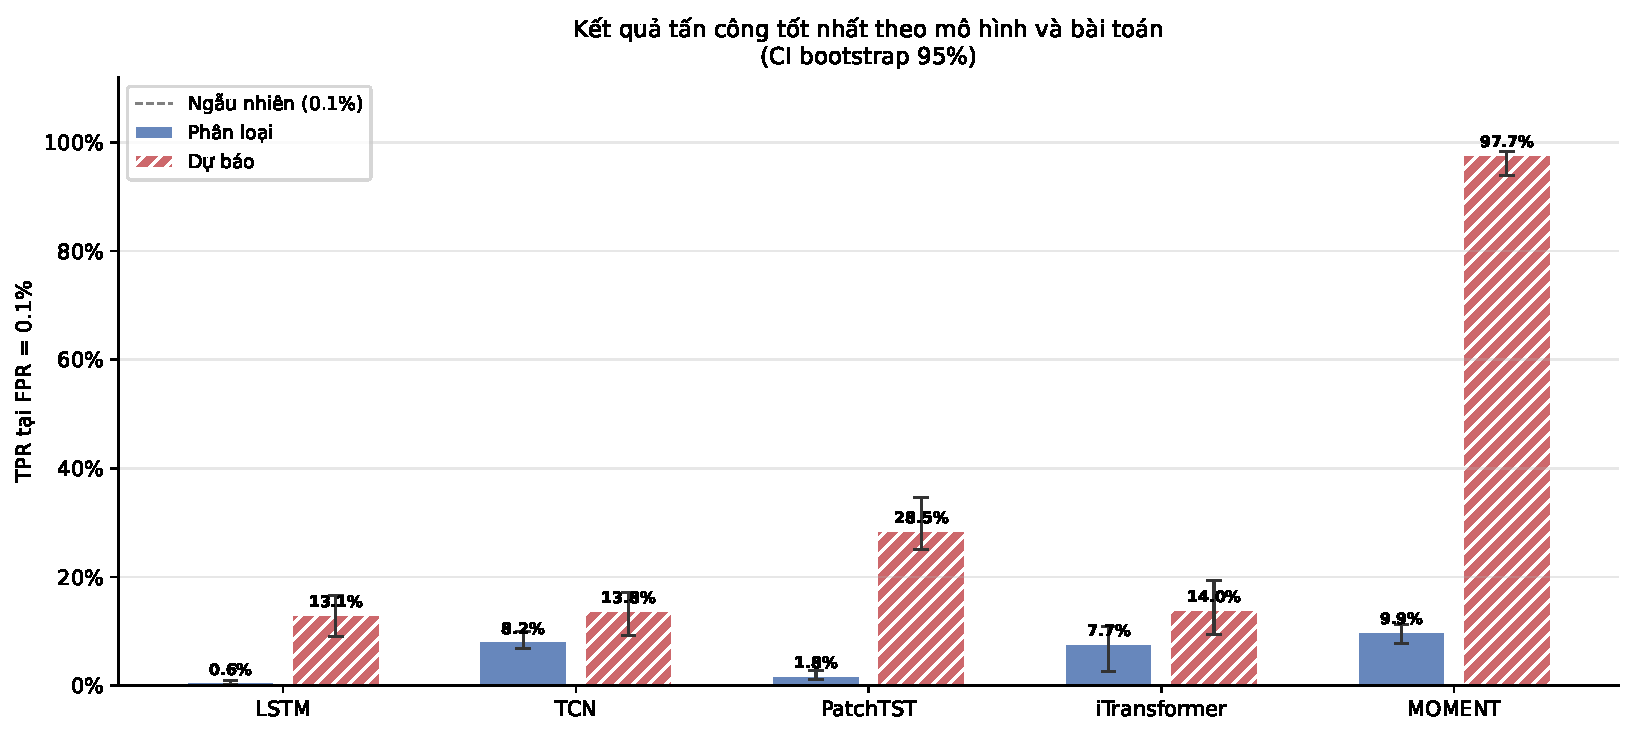
\includegraphics[width=0.88\textwidth]{fig1_best_attack_summary.pdf}
\caption{TPR@0,1\% FPR của tấn công tốt nhất theo mô hình và bài toán (CI bootstrap 95\%). Đường nét đứt = bộ phân loại ngẫu nhiên.}
\label{fig:best_summary}
\end{figure}

\textbf{Phân tích Hình~\ref{fig:best_summary}.} (i) Ở cả năm mô hình, cột dự báo cao hơn cột phân loại. (ii) Trên phân loại, năm mô hình tách thành hai nhóm: LSTM ($0{,}61\%$) và PatchTST ($1{,}84\%$) thấp, còn TCN ($8{,}17\%$), iTransformer ($7{,}73\%$) và MOMENT ($9{,}92\%$) cao hơn $4$--$16$ lần. CI của ba mô hình sau chồng lấn nhau (iTransformer: $[2{,}6\%; 10{,}8\%]$), nên thứ tự giữa chúng không có ý nghĩa thống kê; chỉ phân biệt được nhóm thấp với nhóm cao. (iii) Test accuracy của bốn mô hình LSTM, TCN, PatchTST, MOMENT nằm trong khoảng hẹp $0{,}759$--$0{,}781$ trong khi rò rỉ chênh nhau $\sim 16$ lần ($0{,}61\%$ đến $9{,}92\%$): utility ngang nhau không kéo theo quyền riêng tư ngang nhau. (iv) Trên dự báo, LSTM, TCN và iTransformer tụ lại quanh $13$--$14\%$ dù gap MSE khác nhau rõ ($0{,}25$; $0{,}08$; $0{,}48$), còn PatchTST ($28{,}5\%$) gấp đôi và MOMENT ($97{,}7\%$) là điểm ngoại lai.

\begin{figure}[H]
\centering
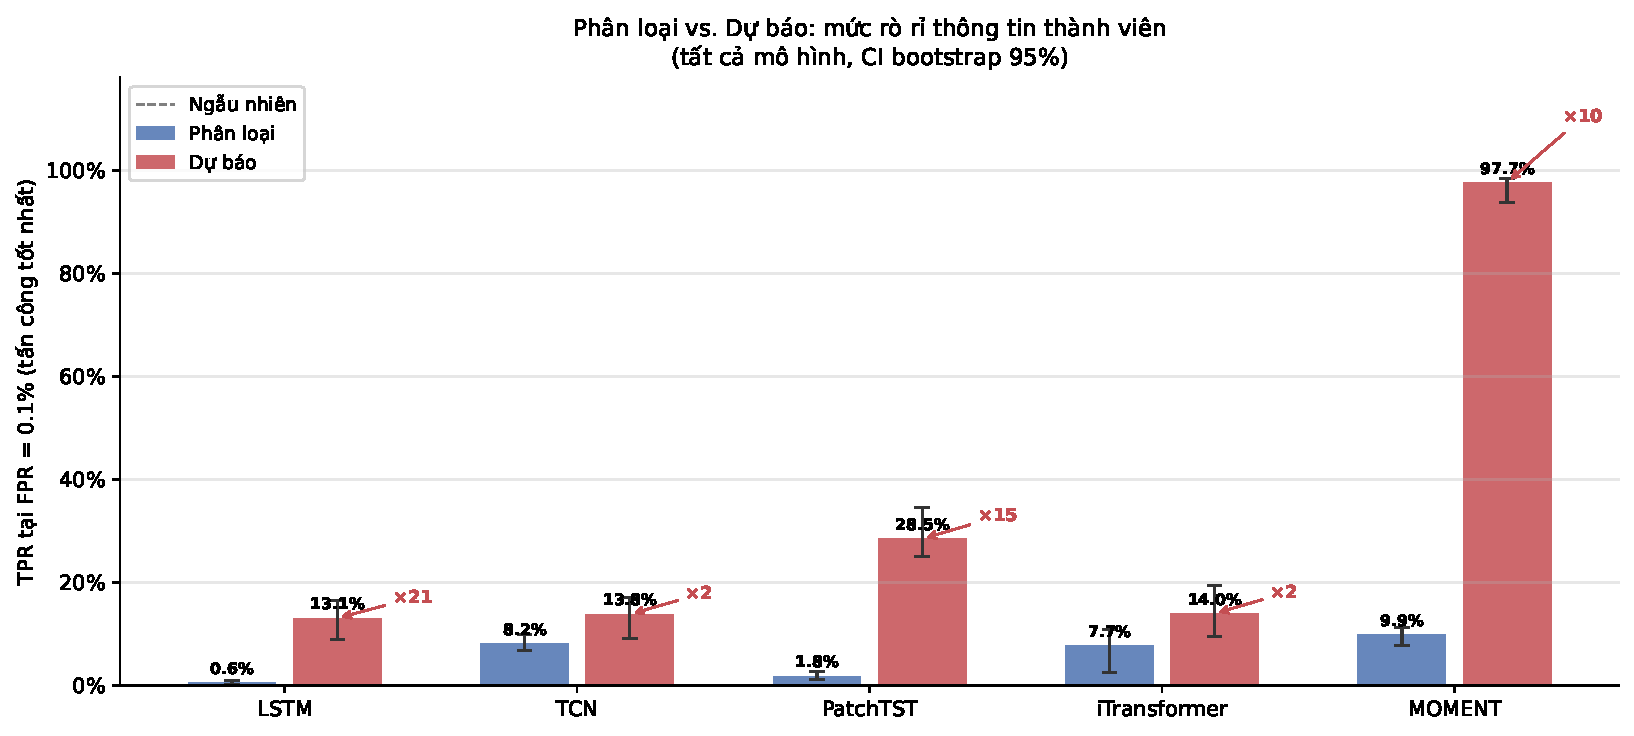
\includegraphics[width=0.88\textwidth]{fig4_cls_vs_fcst.pdf}
\caption{So sánh mức rò rỉ giữa phân loại (xanh) và dự báo (đỏ) cho từng mô hình, sử dụng tấn công tốt nhất. Số bội ($\times$) cho biết dự báo dễ bị tấn công hơn bao nhiêu lần so với phân loại.}
\label{fig:cls_vs_fcst}
\end{figure}

\textbf{Phân tích Hình~\ref{fig:cls_vs_fcst}.} Hệ số nhân phụ thuộc mạnh vào mẫu số: LSTM đạt $21\times$ chỉ vì mẫu số phân loại rất nhỏ ($0{,}61\%$), còn mức tăng tuyệt đối chỉ $+12{,}5$ điểm phần trăm; ngược lại MOMENT ($\approx 10\times$) tăng tới $+87{,}7$ điểm phần trăm. Xét hiệu tuyệt đối, thứ tự là MOMENT ($+87{,}7$) $\gg$ PatchTST ($+26{,}6$) $>$ LSTM ($+12{,}5$) $>$ iTransformer ($+6{,}3$) $\approx$ TCN ($+5{,}7$). Với TCN, CI dự báo $[9{,}2\%; 17{,}1\%]$ tách khỏi CI phân loại $[6{,}8\%; 9{,}9\%]$, nên khác biệt có ý nghĩa; với iTransformer hai CI chồng lấn ($[9{,}4\%; 19{,}4\%]$ so với $[2{,}6\%; 10{,}8\%]$), nên khoảng cách $1{,}8\times$ chưa được chứng minh. Kết luận ``dự báo rò rỉ nhiều hơn'' do đó chắc chắn với LSTM, PatchTST, MOMENT, còn với TCN và iTransformer chỉ ở mức khiêm tốn. Cần nhớ thêm rằng với LSTM, TCN, PatchTST bài toán dự báo được huấn luyện 50 epoch so với 20 epoch của phân loại (Bảng~\ref{tab:hparams}), nên phần chênh lệch có thể lẫn hiệu ứng số epoch.

\section{Kết quả trên PatchTST (TV2: Trần Trọng Hoàng)}

\subsection{Bài toán phân loại}

Bảng~\ref{tab:patchtst_cls} trình bày kết quả trên PatchTST cho phân loại (20 epoch, gap $0{,}133$).

\begin{table}[H]
\centering
\caption{PatchTST -- Phân loại (PTB-XL, 20 epoch). CI: khoảng tin cậy bootstrap 95\% (1.000 lần lấy mẫu) cho TPR@0,1\%.}
\label{tab:patchtst_cls}
\begin{tabular}{lcccc}
\toprule
\textbf{Tấn công} & \textbf{TPR@0,1\%} & \textbf{CI 95\%} & \textbf{TPR@1\%} & \textbf{AUC} \\
\midrule
Loss      & 0,0020 & [0,0002; 0,0030] & 0,0147 & 0,574 \\
Conf      & 0,0020 & [0,0002; 0,0030] & 0,0147 & 0,533 \\
Entropy   & 0,0021 & [0,0002; 0,0031] & 0,0147 & 0,532 \\
LiRA      & 0,0095 & [0,0029; 0,0170] & 0,0452 & 0,645 \\
LiRA-off  & 0,0060 & [0,0021; 0,0146] & 0,0429 & 0,647 \\
RMIA      & 0,0136 & [0,0081; 0,0211] & 0,0565 & 0,653 \\
RMIA-on   & \textbf{0,0184} & [0,0114; 0,0279] & \textbf{0,0735} & \textbf{0,676} \\
Temporal  & 0,0080 & [0,0045; 0,0103] & 0,0404 & 0,631 \\
\midrule
Ngẫu nhiên & 0,0010 & -- & 0,0100 & 0,500 \\
\bottomrule
\end{tabular}
\end{table}

\textbf{Phân tích.} (1) \textit{Tấn công đơn giản gần ngẫu nhiên:} Loss, Conf và Entropy đạt TPR@0,1\% $\approx 0{,}2\%$ (khoảng 16/8.136 member vượt ngưỡng) với cận trên CI $\approx 0{,}3\%$; do cận dưới ($0{,}02\%$) nằm dưới mức ngẫu nhiên, ta không loại được khả năng đây chỉ là nhiễu. Loss có AUC cao hơn (0,574 so với $\approx 0{,}53$) vì dùng nhãn thật, nhưng ở vùng low-FPR ba tấn công trùng TPR, tức cùng dựa vào một nhóm nhỏ mẫu cực đoan. (2) \textit{Hiệu chỉnh theo độ khó có tác dụng:} RMIA-online đạt $1{,}84\%$ (CI $[1{,}14\%; 2{,}79\%]$, cận dưới đã cao hơn mức ngẫu nhiên), gấp $\approx 9\times$ Loss; ở TPR@1\% FPR đạt $7{,}35\%$ ($7\times$ ngẫu nhiên). (3) \textit{Online hơn offline} nhưng không chắc chắn: LiRA $0{,}95\%$ so với LiRA-off $0{,}60\%$, RMIA-online $1{,}84\%$ so với RMIA $1{,}36\%$; các CI chồng lấn một phần. (4) \textit{Temporal không cần shadow vẫn vượt các tấn công đơn giản} ($0{,}80\%$); kết quả ablation trong tệp kết quả cho thấy bộ phân loại chỉ dùng đầu ra epoch cuối chỉ đạt $0{,}04\%$, nghĩa là tín hiệu nằm ở \textit{quỹ đạo} qua các epoch chứ không ở đầu ra cuối. (5) Tổng thể, PatchTST với gap $0{,}133$ rò rỉ yếu: tấn công tốt nhất chỉ gấp $\approx 18\times$ ngẫu nhiên.

\begin{figure}[H]
\centering
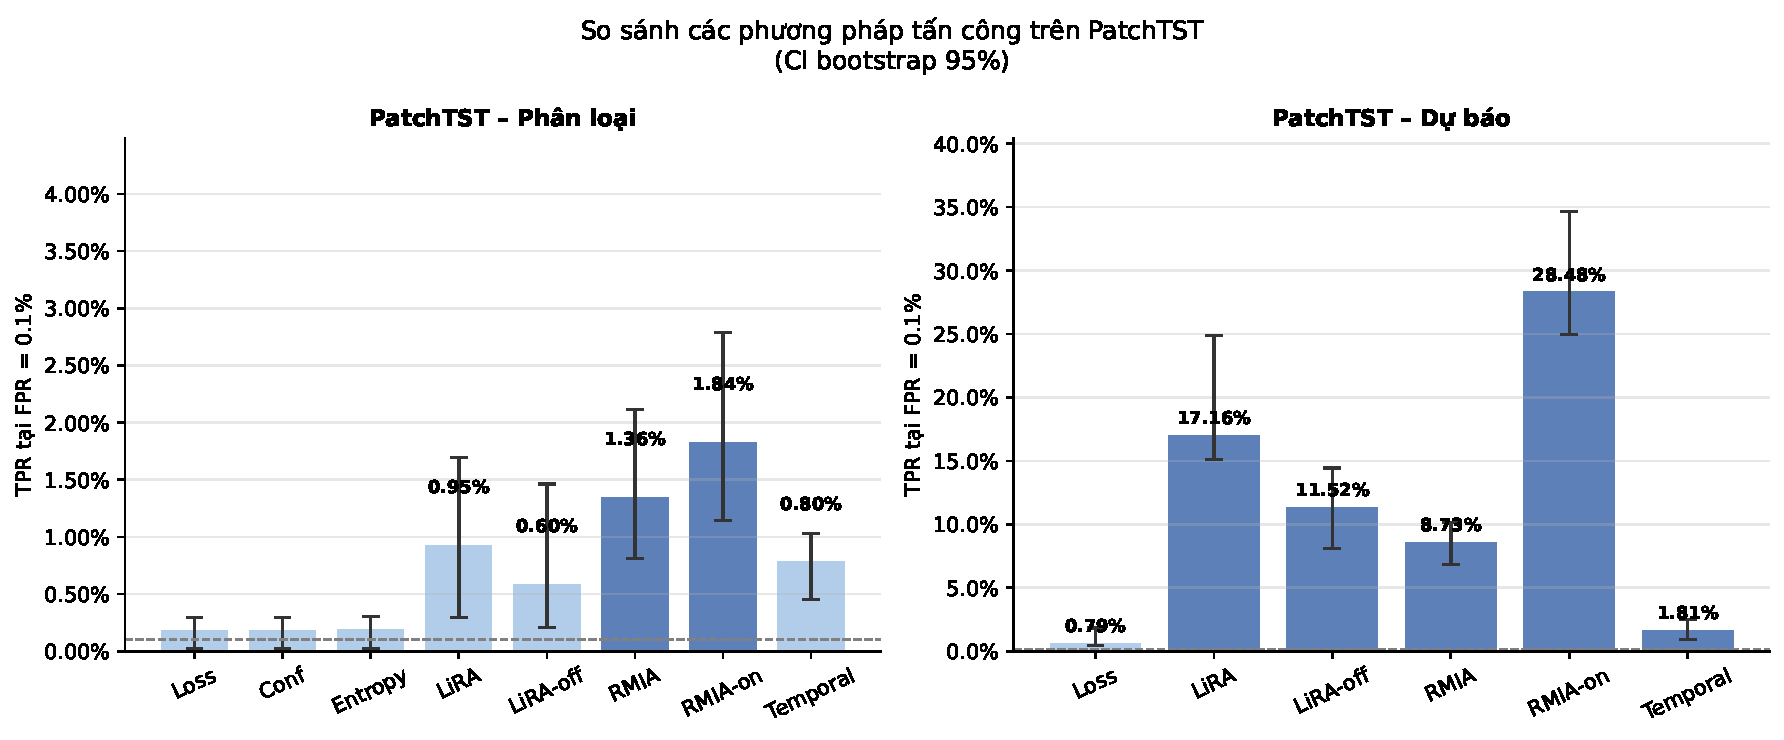
\includegraphics[width=\textwidth]{fig3_patchtst_attacks.pdf}
\caption{TPR@0,1\% FPR của các phương pháp tấn công trên PatchTST: phân loại (trái) và dự báo (phải). Thanh màu nhạt: tấn công gần ngẫu nhiên; thanh màu đậm: tấn công có hiệu quả.}
\label{fig:patchtst_attacks}
\end{figure}

\textbf{Phân tích Hình~\ref{fig:patchtst_attacks}.} Hai panel dùng thang trục y khác nhau (phân loại tối đa vài \%, dự báo tới $\sim 30\%$), nên chỉ so sánh được thứ hạng trong từng panel, không so chiều cao thanh giữa hai panel. Thứ hạng giữa các tấn công \textit{đảo chiều} giữa hai bài toán: ở phân loại RMIA (offline) $>$ LiRA ($1{,}36\%$ so với $0{,}95\%$), còn ở dự báo LiRA $\gg$ RMIA ($17{,}2\%$ so với $8{,}7\%$). Hiện tượng RMIA-offline kém LiRA-online xuất hiện ở bốn trong năm mô hình dự báo (Bảng~\ref{tab:main_attacks}); nguyên nhân có thể là phép biến đổi $p = \exp(-\mathrm{MSE}/\tau)$ nén các mẫu có MSE thấp về gần nhau, song nhóm chưa kiểm chứng giả thuyết này.

\subsection{Bài toán dự báo}

\begin{table}[H]
\centering
\caption{PatchTST -- Dự báo (PTB-XL, $H = 96$, 50 epoch).}
\label{tab:patchtst_fcst}
\begin{tabular}{lcccc}
\toprule
\textbf{Tấn công} & \textbf{TPR@0,1\%} & \textbf{CI 95\%} & \textbf{TPR@1\%} & \textbf{AUC} \\
\midrule
Loss      & 0,0079 & [0,0045; 0,0183] & 0,0653 & 0,694 \\
LiRA      & 0,1716 & [0,1511; 0,2491] & 0,4704 & 0,963 \\
LiRA-off  & 0,1152 & [0,0812; 0,1444] & 0,2663 & 0,899 \\
RMIA      & 0,0873 & [0,0683; 0,1018] & 0,1861 & 0,778 \\
RMIA-on   & \textbf{0,2848} & [0,2500; 0,3462] & \textbf{0,5281} & \textbf{0,966} \\
Temporal  & 0,0181 & [0,0095; 0,0252] & 0,0978 & 0,798 \\
\midrule
Ngẫu nhiên & 0,0010 & -- & 0,0100 & 0,500 \\
\bottomrule
\end{tabular}
\end{table}

\textbf{Phân tích.} (1) Mức rò rỉ tăng mạnh: RMIA-online đạt $28{,}5\%$ (CI $[25{,}0\%; 34{,}6\%]$), LiRA $17{,}2\%$ ($[15{,}1\%; 24{,}9\%]$); hai CI gần như tách nhau nên RMIA-online hơn LiRA khá chắc. (2) AUC của LiRA và RMIA-online gần như bằng nhau ($0{,}963$ và $0{,}966$) nhưng TPR@0,1\% chênh $1{,}7\times$: ở vùng AUC $\ge 0{,}96$, AUC không còn phân biệt được tấn công, đây là lý do tiêu chuẩn low-FPR cần thiết. (3) \textit{Loss một mình} đạt $0{,}79\%$ ($\approx 8\times$ ngẫu nhiên) với AUC $0{,}694$, tức khác với phân loại, tín hiệu rò rỉ đã hiện diện ngay ở MSE thô. (4) Temporal ($1{,}81\%$, AUC $0{,}798$) chỉ nhỉnh hơn bộ phân loại chỉ dùng log-MSE ($0{,}80\%$), nên đặc trưng DFT/xu hướng đóng góp ít trên PatchTST, khác hẳn MOMENT (Mục~\ref{sec:moment_analysis}). (5) Gap MSE $0{,}175$ (test cao hơn train $\approx 25\%$) đã đủ để một tấn công hiệu chỉnh theo độ khó cho TPR $\approx 285\times$ mức ngẫu nhiên.

\section{Kết quả trên LSTM và TCN -- Baseline (TV1: Bùi Lê Hoài An)}

\subsection{LSTM}

\begin{table}[H]
\centering
\caption{LSTM -- Phân loại (PTB-XL, 20 epoch).}
\label{tab:lstm_cls}
\begin{tabular}{lcccc}
\toprule
\textbf{Tấn công} & \textbf{TPR@0,1\%} & \textbf{CI 95\%} & \textbf{TPR@1\%} & \textbf{AUC} \\
\midrule
Loss      & 0,0016 & [0,0005; 0,0029] & 0,0129 & 0,530 \\
Conf      & 0,0016 & [0,0005; 0,0029] & 0,0129 & 0,509 \\
Entropy   & 0,0017 & [0,0005; 0,0028] & 0,0125 & 0,510 \\
LiRA      & 0,0038 & [0,0021; 0,0061] & 0,0261 & 0,563 \\
LiRA-off  & \textbf{0,0061} & [0,0022; 0,0097] & 0,0270 & 0,568 \\
RMIA      & 0,0045 & [0,0022; 0,0074] & 0,0263 & 0,564 \\
RMIA-on   & 0,0053 & [0,0036; 0,0080] & \textbf{0,0320} & \textbf{0,582} \\
Temporal  & 0,0009 & [0,0002; 0,0027] & 0,0127 & 0,547 \\
\midrule
Ngẫu nhiên & 0,0010 & -- & 0,0100 & 0,500 \\
\bottomrule
\end{tabular}
\end{table}

\begin{table}[H]
\centering
\caption{LSTM -- Dự báo (PTB-XL, $H = 96$, 50 epoch).}
\label{tab:lstm_fcst}
\begin{tabular}{lcccc}
\toprule
\textbf{Tấn công} & \textbf{TPR@0,1\%} & \textbf{CI 95\%} & \textbf{TPR@1\%} & \textbf{AUC} \\
\midrule
Loss      & 0,0182 & [0,0079; 0,0245] & 0,0841 & 0,772 \\
LiRA      & 0,0874 & [0,0664; 0,1436] & 0,3201 & 0,955 \\
LiRA-off  & 0,0510 & [0,0240; 0,0846] & 0,2081 & 0,898 \\
RMIA      & 0,0600 & [0,0517; 0,0816] & 0,2113 & 0,857 \\
RMIA-on   & \textbf{0,1309} & [0,0896; 0,1657] & \textbf{0,4302} & \textbf{0,958} \\
Temporal  & 0,0123 & [0,0049; 0,0277] & 0,1019 & 0,824 \\
\midrule
Ngẫu nhiên & 0,0010 & -- & 0,0100 & 0,500 \\
\bottomrule
\end{tabular}
\end{table}

\begin{figure}[H]
\centering
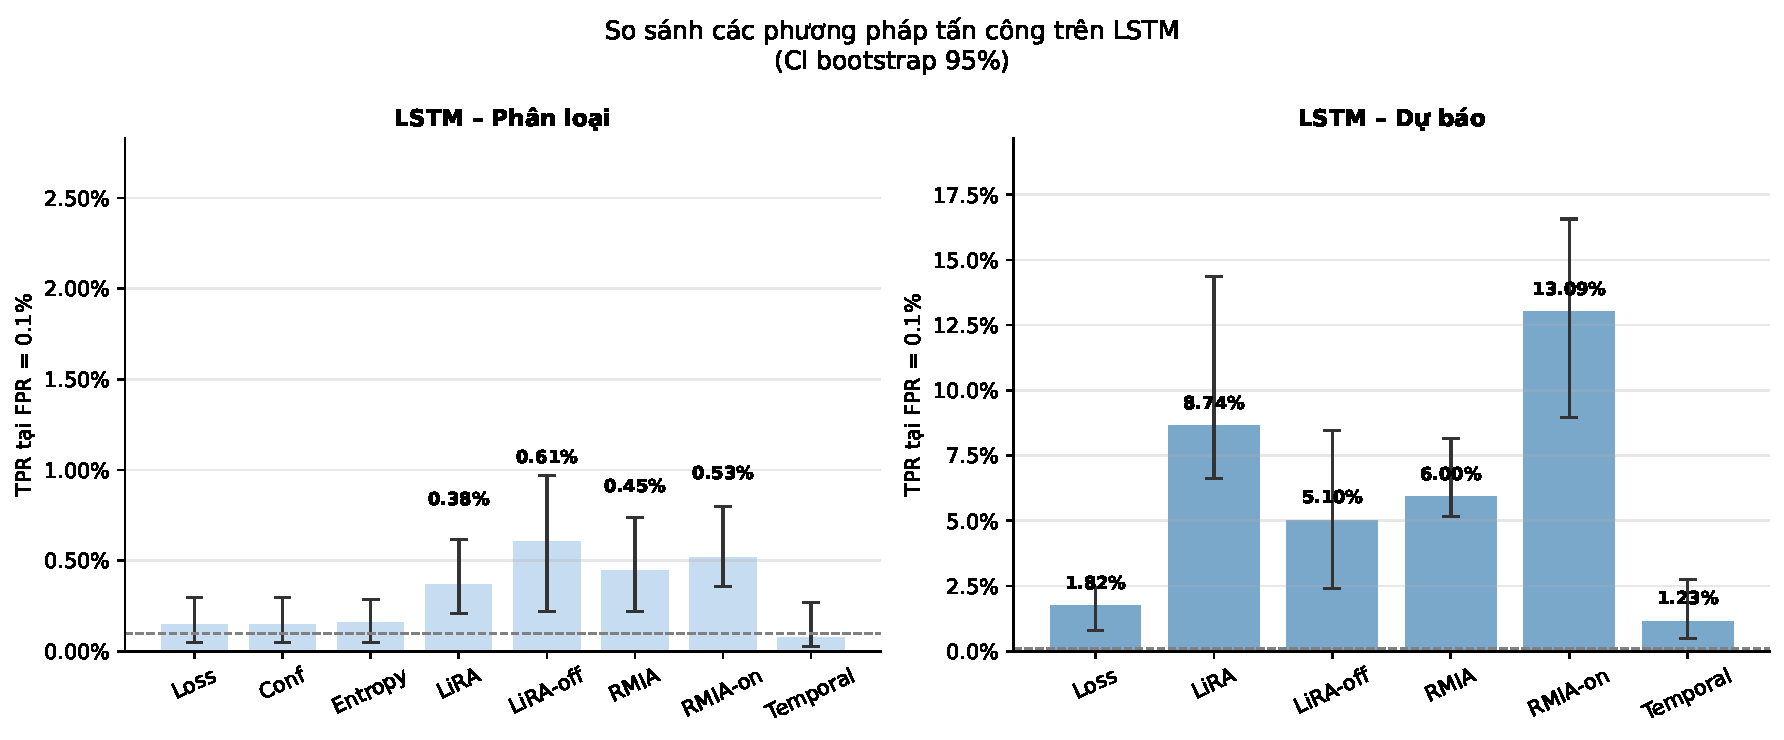
\includegraphics[width=\textwidth]{fig5_lstm_attacks.pdf}
\caption{TPR@0,1\% FPR của các phương pháp tấn công trên LSTM: phân loại (trái) và dự báo (phải).}
\label{fig:lstm_attacks}
\end{figure}

\textbf{Phân tích Bảng~\ref{tab:lstm_cls} và Hình~\ref{fig:lstm_attacks}.} LSTM có gap phân loại nhỏ nhất ($0{,}052$; train $0{,}833$, test $0{,}781$) và cũng là mô hình rò rỉ ít nhất ($0{,}61\%$ với LiRA-offline, $0{,}53\%$ với RMIA-online). Chỉ các tấn công dựa trên shadow có cận dưới CI vượt $0{,}1\%$ (LiRA $[0{,}21\%; 0{,}61\%]$); Loss, Conf, Entropy và Temporal ($0{,}09\%$, thấp hơn cả mức ngẫu nhiên) không khác biệt có ý nghĩa so với đoán mò. Ở phân loại, LiRA-offline ($0{,}61\%$) cao hơn LiRA-online ($0{,}38\%$), ngược với chiều thông thường, nhưng khác biệt nằm trong nhiễu của CI.

\textbf{Phân tích Bảng~\ref{tab:lstm_fcst}.} Trên dự báo, gap MSE là $0{,}250$ (train $0{,}646$, test $0{,}897$, lớn nhất trong ba mô hình huấn luyện từ đầu có utility bình thường) và RMIA-online đạt $13{,}1\%$ ($131\times$ ngẫu nhiên, CI $[9{,}0\%; 16{,}6\%]$). Khoảng cách online--offline rõ rệt: RMIA-online $13{,}1\%$ so với RMIA $6{,}0\%$, LiRA $8{,}7\%$ so với LiRA-off $5{,}1\%$, tức biết bản ghi mục tiêu nằm trong nhóm IN của shadow làm tăng $\approx 1{,}7$--$2{,}2\times$ TPR. AUC đạt $0{,}955$--$0{,}958$ ở LiRA và RMIA-online nhưng TPR@0,1\% chỉ $8{,}7$--$13{,}1\%$, minh họa khoảng cách giữa AUC và hiệu năng low-FPR.

\subsection{TCN}

\begin{table}[H]
\centering
\caption{TCN -- Phân loại (PTB-XL, 20 epoch).}
\label{tab:tcn_cls}
\begin{tabular}{lcccc}
\toprule
\textbf{Tấn công} & \textbf{TPR@0,1\%} & \textbf{CI 95\%} & \textbf{TPR@1\%} & \textbf{AUC} \\
\midrule
Loss      & 0,0007 & [0,0000; 0,0017] & 0,0108 & 0,628 \\
Conf      & 0,0007 & [0,0000; 0,0017] & 0,0108 & 0,578 \\
Entropy   & 0,0007 & [0,0000; 0,0017] & 0,0108 & 0,577 \\
LiRA      & 0,0457 & [0,0385; 0,0605] & 0,1289 & 0,751 \\
LiRA-off  & 0,0256 & [0,0134; 0,0423] & 0,1160 & 0,709 \\
RMIA      & 0,0520 & [0,0333; 0,0644] & 0,1377 & 0,745 \\
RMIA-on   & \textbf{0,0817} & [0,0680; 0,0993] & \textbf{0,1659} & \textbf{0,758} \\
Temporal  & 0,0216 & [0,0088; 0,0337] & 0,0919 & 0,736 \\
\midrule
Ngẫu nhiên & 0,0010 & -- & 0,0100 & 0,500 \\
\bottomrule
\end{tabular}
\end{table}

\begin{table}[H]
\centering
\caption{TCN -- Dự báo (PTB-XL, $H = 96$, 50 epoch). RMIA-on suy biến (Mục~\ref{sec:artifacts}).}
\label{tab:tcn_fcst}
\begin{tabular}{lcccc}
\toprule
\textbf{Tấn công} & \textbf{TPR@0,1\%} & \textbf{CI 95\%} & \textbf{TPR@1\%} & \textbf{AUC} \\
\midrule
Loss      & 0,0044 & [0,0028; 0,0087] & 0,0311 & 0,607 \\
LiRA      & \textbf{0,1383} & [0,0919; 0,1707] & \textbf{0,3741} & \textbf{0,936} \\
LiRA-off  & 0,0882 & [0,0520; 0,1310] & 0,2845 & 0,903 \\
RMIA      & 0,0176 & [0,0088; 0,0216] & 0,0758 & 0,670 \\
RMIA-on   & 0,0395 & [0,0354; 0,0438] & 0,0395 & 0,520 \\
Temporal  & 0,0070 & [0,0007; 0,0128] & 0,0429 & 0,673 \\
\midrule
Ngẫu nhiên & 0,0010 & -- & 0,0100 & 0,500 \\
\bottomrule
\end{tabular}
\end{table}

\begin{figure}[H]
\centering
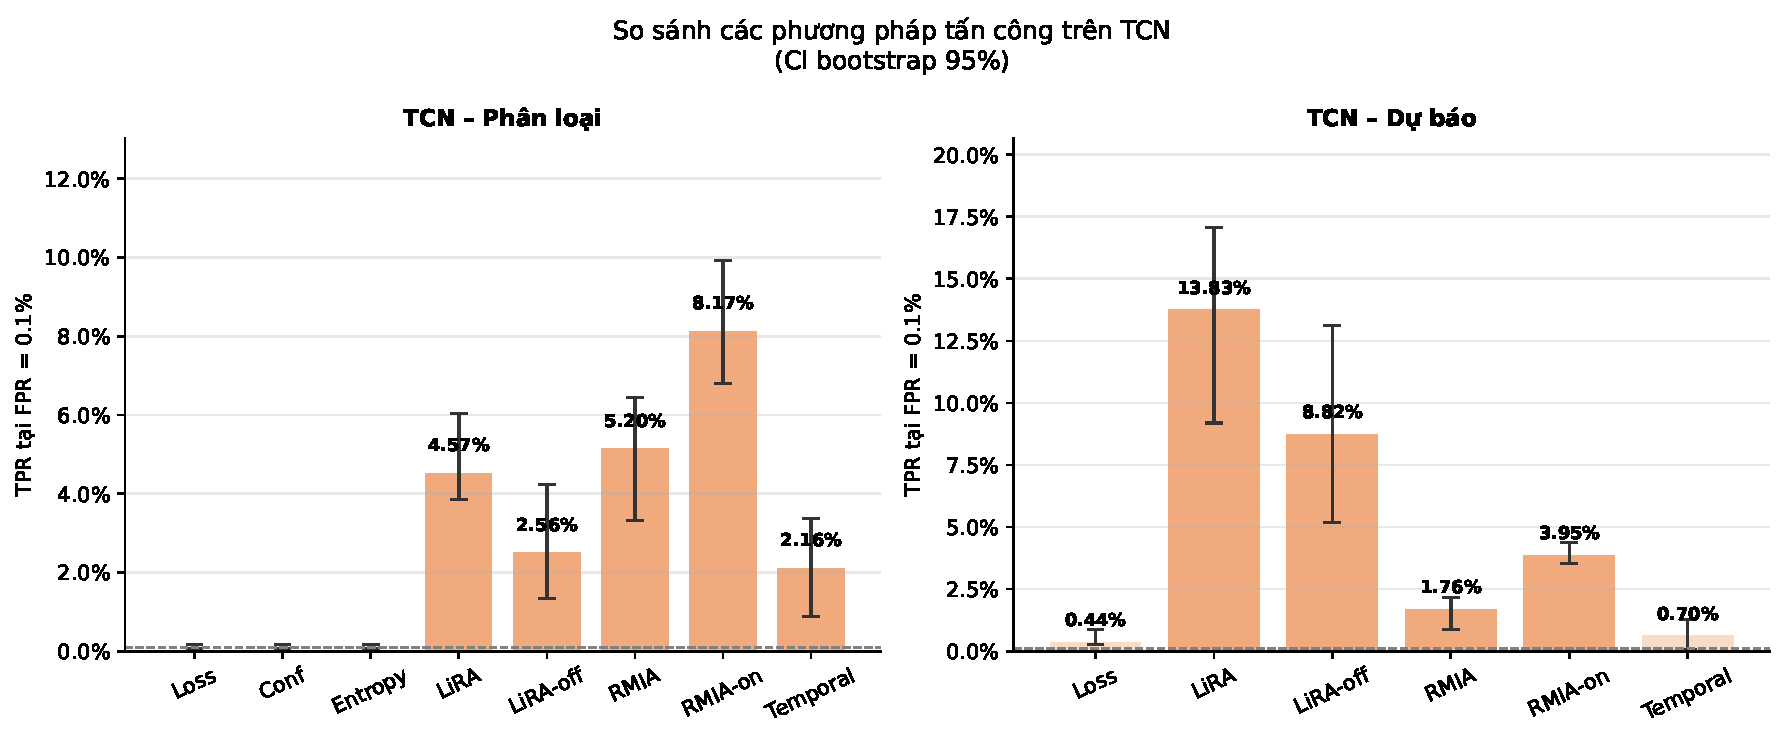
\includegraphics[width=\textwidth]{fig6_tcn_attacks.pdf}
\caption{TPR@0,1\% FPR của các phương pháp tấn công trên TCN: phân loại (trái) và dự báo (phải). TCN phân loại rò rỉ nhiều hơn LSTM (RMIA-on $= 8{,}17\%$); trên dự báo RMIA-on suy biến (Mục~\ref{sec:artifacts}).}
\label{fig:tcn_attacks}
\end{figure}

\textbf{Phân tích Bảng~\ref{tab:tcn_cls} và Hình~\ref{fig:tcn_attacks} (trái).} TCN có gap phân loại lớn nhất trong nhóm có utility bình thường ($0{,}213$: train $0{,}973$, test $0{,}759$), tương ứng RMIA-online $8{,}17\%$ (CI $[6{,}8\%; 9{,}9\%]$), LiRA $4{,}57\%$ và Temporal $2{,}16\%$; so với LSTM (gap $0{,}052$) chênh $\approx 13\times$. Đây là bằng chứng mạnh nhất trong dữ liệu cho mối liên hệ gap--rò rỉ ở phân loại. Đáng chú ý, Loss/Conf/Entropy chỉ đạt $0{,}07\%$ (thấp hơn cả ngẫu nhiên) dù AUC của Loss là $0{,}628$: có thể do khi train accuracy $97\%$, nhiều member có loss rất nhỏ và các non-member được dự đoán đúng cũng vậy, nên điểm số thô không tách được ở vùng FPR cực thấp, trong khi tấn công hiệu chỉnh theo độ khó thì tách được (nhóm chưa kiểm tra phân phối điểm số của TCN).

\textbf{Phân tích Bảng~\ref{tab:tcn_fcst} và Hình~\ref{fig:tcn_attacks} (phải).} TCN có gap MSE \textit{nhỏ nhất} trong năm mô hình ($0{,}080$) nhưng LiRA vẫn đạt $13{,}8\%$ (AUC $0{,}936$), trong khi Loss chỉ $0{,}44\%$. Hai quan sát này cho thấy rò rỉ ở dự báo không đi cùng gap trung bình: hiệu chỉnh theo độ khó từng mẫu (shadow) khai thác được ghi nhớ cục bộ mà MSE thô che lấp. RMIA-online ($3{,}95\%$, AUC $0{,}520$) là kết quả suy biến, không phản ánh sức mạnh thật của tấn công (Mục~\ref{sec:artifacts}); tấn công tốt nhất có ý nghĩa là LiRA.

\section{Kết quả trên iTransformer (TV3: Cao Anh Tuấn)}
\label{sec:itrans_analysis}

\begin{table}[H]
\centering
\caption{iTransformer -- Phân loại (PTB-XL, 50 epoch, test accuracy 0,520).}
\label{tab:itrans_cls}
\begin{tabular}{lcccc}
\toprule
\textbf{Tấn công} & \textbf{TPR@0,1\%} & \textbf{CI 95\%} & \textbf{TPR@1\%} & \textbf{AUC} \\
\midrule
Loss      & 0,0000 & [0,0000; 0,0000] & 0,0000 & 0,897 \\
Conf      & 0,0000 & [0,0000; 0,0000] & 0,0000 & 0,857 \\
Entropy   & 0,0057 & [0,0014; 0,0140] & 0,0919 & 0,895 \\
LiRA      & 0,0076 & [0,0032; 0,0143] & 0,0603 & 0,584 \\
LiRA-off  & 0,0375 & [0,0263; 0,0745] & 0,1673 & 0,593 \\
RMIA      & 0,0127 & [0,0074; 0,0234] & 0,0956 & 0,650 \\
RMIA-on   & 0,0118 & [0,0071; 0,0224] & 0,0948 & 0,649 \\
Temporal  & \textbf{0,0773} & [0,0258; 0,1082] & \textbf{0,2710} & \textbf{0,945} \\
\midrule
Ngẫu nhiên & 0,0010 & -- & 0,0100 & 0,500 \\
\bottomrule
\end{tabular}
\end{table}

\begin{table}[H]
\centering
\caption{iTransformer -- Dự báo (PTB-XL, $H = 96$, 50 epoch).}
\label{tab:itrans_fcst}
\begin{tabular}{lcccc}
\toprule
\textbf{Tấn công} & \textbf{TPR@0,1\%} & \textbf{CI 95\%} & \textbf{TPR@1\%} & \textbf{AUC} \\
\midrule
Loss      & 0,0299 & [0,0220; 0,0604] & 0,1645 & 0,911 \\
LiRA      & 0,0106 & [0,0066; 0,0155] & 0,0651 & 0,806 \\
LiRA-off  & 0,0130 & [0,0079; 0,0252] & 0,0950 & 0,823 \\
RMIA      & 0,0116 & [0,0055; 0,0255] & 0,0939 & 0,872 \\
RMIA-on   & 0,0011 & [0,0005; 0,0034] & 0,0386 & 0,843 \\
Temporal  & \textbf{0,1400} & [0,0944; 0,1938] & \textbf{0,4586} & \textbf{0,963} \\
\midrule
Ngẫu nhiên & 0,0010 & -- & 0,0100 & 0,500 \\
\bottomrule
\end{tabular}
\end{table}

\begin{figure}[H]
\centering
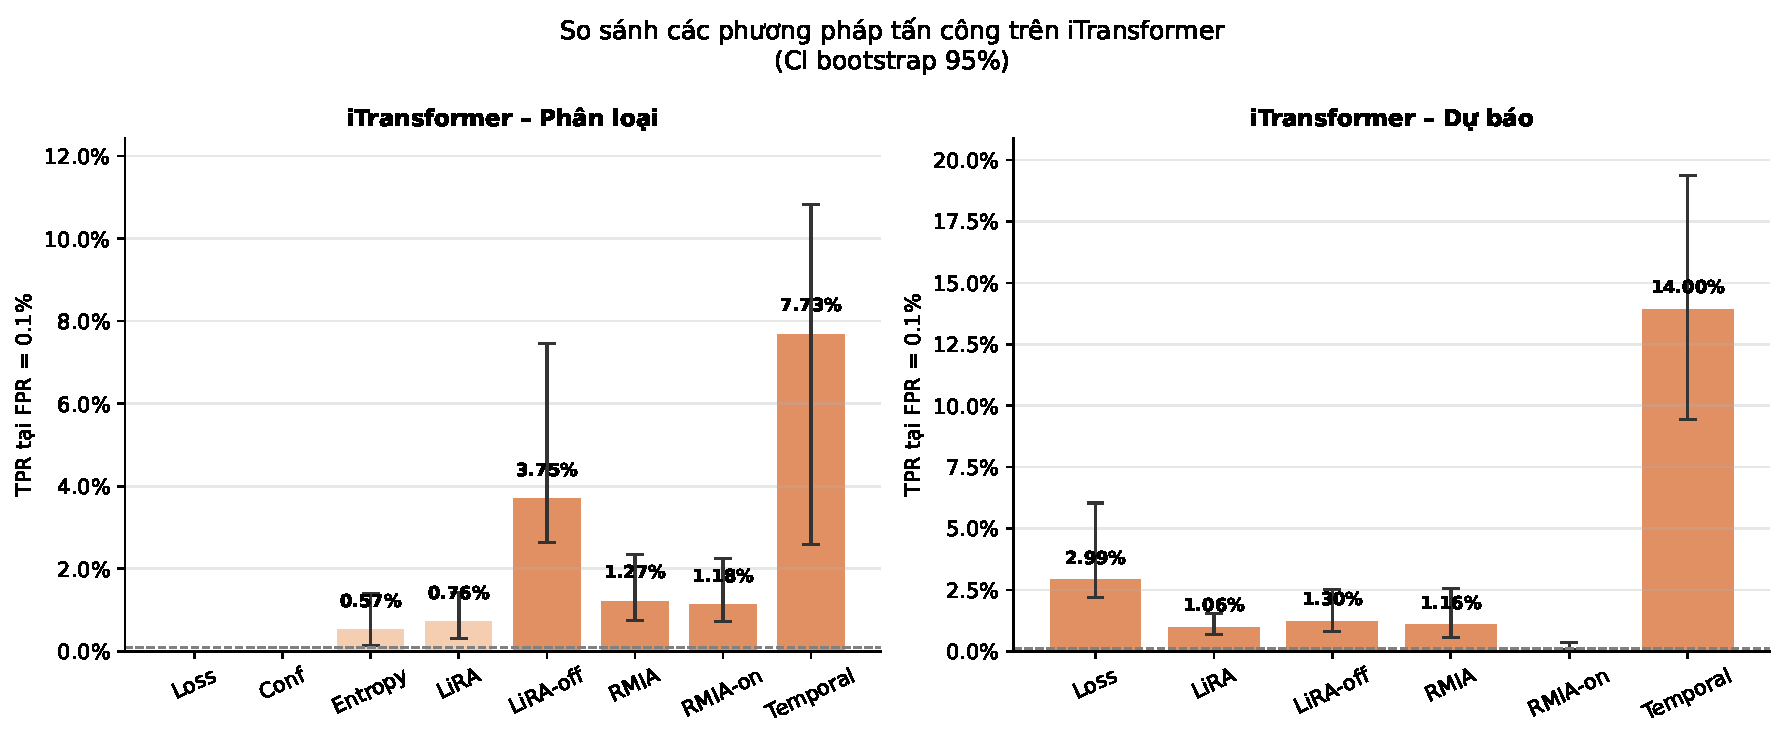
\includegraphics[width=\textwidth]{fig7_itransformer_attacks.pdf}
\caption{TPR@0,1\% FPR của các phương pháp tấn công trên iTransformer: phân loại (trái) và dự báo (phải). Temporal Feature là tấn công tốt nhất trên cả hai bài toán.}
\label{fig:itransformer_attacks}
\end{figure}

\textbf{Phân tích phân loại (Bảng~\ref{tab:itrans_cls}, Hình~\ref{fig:itransformer_attacks} trái).} iTransformer ở trạng thái overfit cực đoan: train accuracy $0{,}9999$ nhưng test chỉ $0{,}520$. Ba hiện tượng đáng chú ý. (1) \textit{Bão hòa điểm số:} Loss và Conf cho AUC $0{,}897$/$0{,}857$ nhưng TPR@1\% FPR $= 0$. Kiểm tra điểm số cho thấy $97{,}2\%$ member có $-\mathrm{CE} = 0$ chính xác, và $22{,}3\%$ non-member cũng ở đúng giá trị đó; do đó chỉ cần hạ ngưỡng xuống mức này là FPR nhảy từ 0 lên $22\%$, và mọi ngưỡng có FPR $\le 1\%$ phải đứng trên giá trị bão hòa nên bỏ qua toàn bộ member (TPR $= 0$). AUC cao phản ánh việc $97\%$ member so với $22\%$ non-member nằm ở mức tối đa, không phản ánh khả năng tấn công ở low-FPR. (2) \textit{LiRA/RMIA yếu:} LiRA $0{,}76\%$ và RMIA $\approx 1{,}2\%$, thấp hơn nhiều so với TCN hay MOMENT dù gap lớn hơn ($0{,}480$). Một cách giải thích hợp lý là logit $\phi = \log\frac{p}{1-p}$ của các shadow cũng bão hòa, khiến phân phối IN và OUT khó tách; nhóm chưa kiểm chứng trực tiếp. (3) \textit{Temporal hiệu quả nhất} ($7{,}73\%$, AUC $0{,}945$, CI $[2{,}6\%; 10{,}8\%]$). Ablation trong tệp kết quả cho thấy bộ phân loại chỉ dùng epoch cuối đạt $2{,}2\%$ và chỉ dùng loss chỉ $0\%$, còn dùng quỹ đạo qua bốn checkpoint ($5, 10, 25, 50$) đạt $7{,}7\%$: tín hiệu nằm ở \textit{động lực học huấn luyện}, không phải ở đặc trưng tần số của đầu vào hay cơ chế inverted attention. CI rất rộng và Temporal là tấn công gray-box cần checkpoint trung gian, nên không nên so trực tiếp với các tấn công black-box khác.

\textbf{Phân tích dự báo (Bảng~\ref{tab:itrans_fcst}).} Gap MSE rất lớn ($0{,}477$; train $0{,}351$, test $0{,}828$) song LiRA/RMIA chỉ đạt $\approx 1\%$ và RMIA-online $0{,}11\%$ (bằng mức ngẫu nhiên). Ngược lại Loss đạt $2{,}99\%$ (AUC $0{,}911$) và Temporal $14{,}0\%$ (CI $[9{,}4\%; 19{,}4\%]$). Bộ phân loại chỉ dùng log-MSE đạt $2{,}8\%$ trong khi thêm DFT, xu hướng và độ trôi của phần dư lên $14{,}0\%$: ở dự báo, thông tin rò rỉ chủ yếu nằm ở \textit{hình dạng phổ của phần dư}, không phải độ lớn sai số. Việc các tấn công dùng shadow thất bại dù mô hình overfit rất mạnh gợi ý shadow (cùng công thức huấn luyện) có hành vi khác mô hình đích (utility kém, nhạy với tập huấn luyện), làm phân phối $\phi$ của shadow không còn đại diện cho mô hình đích.

\textbf{Hệ quả cho RQ1.} iTransformer là phản ví dụ của ``gap quyết định rò rỉ'': gap lớn nhất nhưng tấn công black-box mạnh nhất chỉ $\approx 1\%$ ở phân loại. Do utility kém, kết quả iTransformer nên được xem là chặn dưới đối với các tấn công black-box.

\section{Kết quả trên MOMENT -- Foundation Model (TV4: Lê Thành Ngọc)}
\label{sec:moment_analysis}

\subsection{Bài toán phân loại}

\begin{table}[H]
\centering
\caption{MOMENT (full fine-tune) -- Phân loại (PTB-XL, 10 epoch).}
\label{tab:moment_cls}
\begin{tabular}{lcccc}
\toprule
\textbf{Tấn công} & \textbf{TPR@0,1\%} & \textbf{CI 95\%} & \textbf{TPR@1\%} & \textbf{AUC} \\
\midrule
Loss      & 0,0012 & [0,0004; 0,0021] & 0,0098 & 0,617 \\
Conf      & 0,0012 & [0,0004; 0,0021] & 0,0098 & 0,581 \\
Entropy   & 0,0022 & [0,0007; 0,0038] & 0,0102 & 0,580 \\
LiRA      & 0,0493 & [0,0151; 0,0752] & 0,1619 & 0,749 \\
LiRA-off  & 0,0511 & [0,0176; 0,0726] & 0,1406 & 0,726 \\
RMIA      & 0,0649 & [0,0338; 0,0827] & 0,1497 & 0,737 \\
RMIA-on   & \textbf{0,0992} & [0,0778; 0,1123] & \textbf{0,1724} & \textbf{0,758} \\
Temporal  & 0,0240 & [0,0181; 0,0382] & 0,0835 & 0,702 \\
\midrule
Ngẫu nhiên & 0,0010 & -- & 0,0100 & 0,500 \\
\bottomrule
\end{tabular}
\end{table}

\textbf{Phân tích.} (1) Loss/Conf/Entropy vẫn ở mức ngẫu nhiên ($0{,}12$--$0{,}22\%$, CI chứa $0{,}1\%$) dù MOMENT có train accuracy $0{,}956$. (2) Các tấn công shadow rò rỉ rõ: RMIA-online $9{,}92\%$ (CI $[7{,}8\%; 11{,}2\%]$), RMIA $6{,}49\%$, LiRA $4{,}93\%$, LiRA-off $5{,}11\%$. CI của LiRA và LiRA-off rộng ($[1{,}5\%; 7{,}5\%]$ và $[1{,}8\%; 7{,}3\%]$) và trùng nhau, nên khác biệt online--offline không đáng tin ở mô hình này. (3) Temporal đạt $2{,}40\%$ trong khi bộ phân loại chỉ dùng epoch cuối chỉ $0{,}04\%$; tín hiệu đến từ quỹ đạo qua các epoch $1, 2, 5, 10$. (4) So với PatchTST, RMIA-online cao hơn $5{,}4\times$ ($9{,}92\%$ so với $1{,}84\%$) nhưng chỉ ngang TCN ($8{,}17\%$) và iTransformer; CI của MOMENT $[7{,}8\%; 11{,}2\%]$ chồng lấn CI của TCN $[6{,}8\%; 9{,}9\%]$, nên chưa thể kết luận MOMENT rò rỉ hơn mọi mô hình huấn luyện từ đầu ở phân loại.

\paragraph{Phụ thuộc vào số epoch.} Bảng~\ref{tab:epoch} ghi lại utility và tấn công Loss tại các epoch đánh giá (chỉ Loss được tính theo từng epoch; các tấn công shadow chỉ tính ở epoch cuối).

\begin{table}[H]
\centering
\caption{MOMENT: gap và tấn công Loss theo epoch (full fine-tune). Phân loại: gap = train $-$ test accuracy; dự báo: gap = test $-$ train MSE.}
\label{tab:epoch}
\begin{tabular}{lcccccc}
\toprule
 & \multicolumn{3}{c}{\textbf{Phân loại}} & \multicolumn{3}{c}{\textbf{Dự báo}} \\
\cmidrule(lr){2-4}\cmidrule(lr){5-7}
\textbf{Epoch} & Gap & TPR@0,1\% & AUC & Gap & TPR@0,1\% & AUC \\
\midrule
1  & $-0{,}002$ & 0,0014 & 0,507 & 0,014 & 0,0018 & 0,514 \\
2  & $0{,}011$  & 0,0007 & 0,507 & 0,029 & 0,0011 & 0,530 \\
5  & $0{,}026$  & 0,0010 & 0,525 & 0,154 & 0,0039 & 0,671 \\
10 & $0{,}179$  & 0,0012 & 0,617 & 0,446 & 0,0222 & 0,913 \\
\bottomrule
\end{tabular}
\end{table}

\textbf{Phân tích Bảng~\ref{tab:epoch}.} Rò rỉ không tăng tuyến tính theo epoch mà bùng nổ ở cuối quá trình: ở phân loại, gap chỉ $0{,}026$ tại epoch 5 rồi nhảy lên $0{,}179$ tại epoch 10 (train accuracy từ $0{,}784$ lên $0{,}956$) trùng với giai đoạn learning rate được hạ dần của OneCycleLR; AUC của Loss từ $0{,}525$ lên $0{,}617$. Ở dự báo, gap tăng $\approx 3\times$ từ epoch 5 đến 10 ($0{,}154 \to 0{,}446$), AUC từ $0{,}671$ lên $0{,}913$ và TPR@0,1\% từ $0{,}39\%$ lên $2{,}2\%$. Hệ quả: (a) MIA phụ thuộc rất mạnh vào giai đoạn cuối với lịch OneCycleLR; (b) ``10 epoch ít hơn 20 epoch của PatchTST'' không đồng nghĩa ít ghi nhớ, vì mức ghi nhớ gắn với gap chứ không với số epoch; (c) vì chỉ có một tập epoch $\{1, 2, 5, 10\}$ và một lịch LR, ta không tách được ảnh hưởng của số epoch khỏi ảnh hưởng của learning rate.

\subsection{Bài toán dự báo}

\begin{table}[H]
\centering
\caption{MOMENT (full fine-tune) -- Dự báo (PTB-XL, $H = 96$, 10 epoch).}
\label{tab:moment_fcst}
\begin{tabular}{lcccc}
\toprule
\textbf{Tấn công} & \textbf{TPR@0,1\%} & \textbf{CI 95\%} & \textbf{TPR@1\%} & \textbf{AUC} \\
\midrule
Loss      & 0,0222 & [0,0108; 0,0532] & 0,1826 & 0,913 \\
LiRA      & 0,9442 & [0,8358; 0,9864] & 0,9985 & 0,9997 \\
LiRA-off  & 0,8305 & [0,6701; 0,9141] & 0,9791 & 0,9988 \\
RMIA      & 0,7216 & [0,5827; 0,7484] & 0,8616 & 0,987 \\
RMIA-on   & \textbf{0,9765} & [0,9384; 0,9833] & \textbf{0,9986} & \textbf{0,9999} \\
Temporal  & 0,3037 & [0,2467; 0,3780] & 0,6147 & 0,975 \\
\midrule
Ngẫu nhiên & 0,0010 & -- & 0,0100 & 0,500 \\
\bottomrule
\end{tabular}
\end{table}

\begin{figure}[H]
\centering
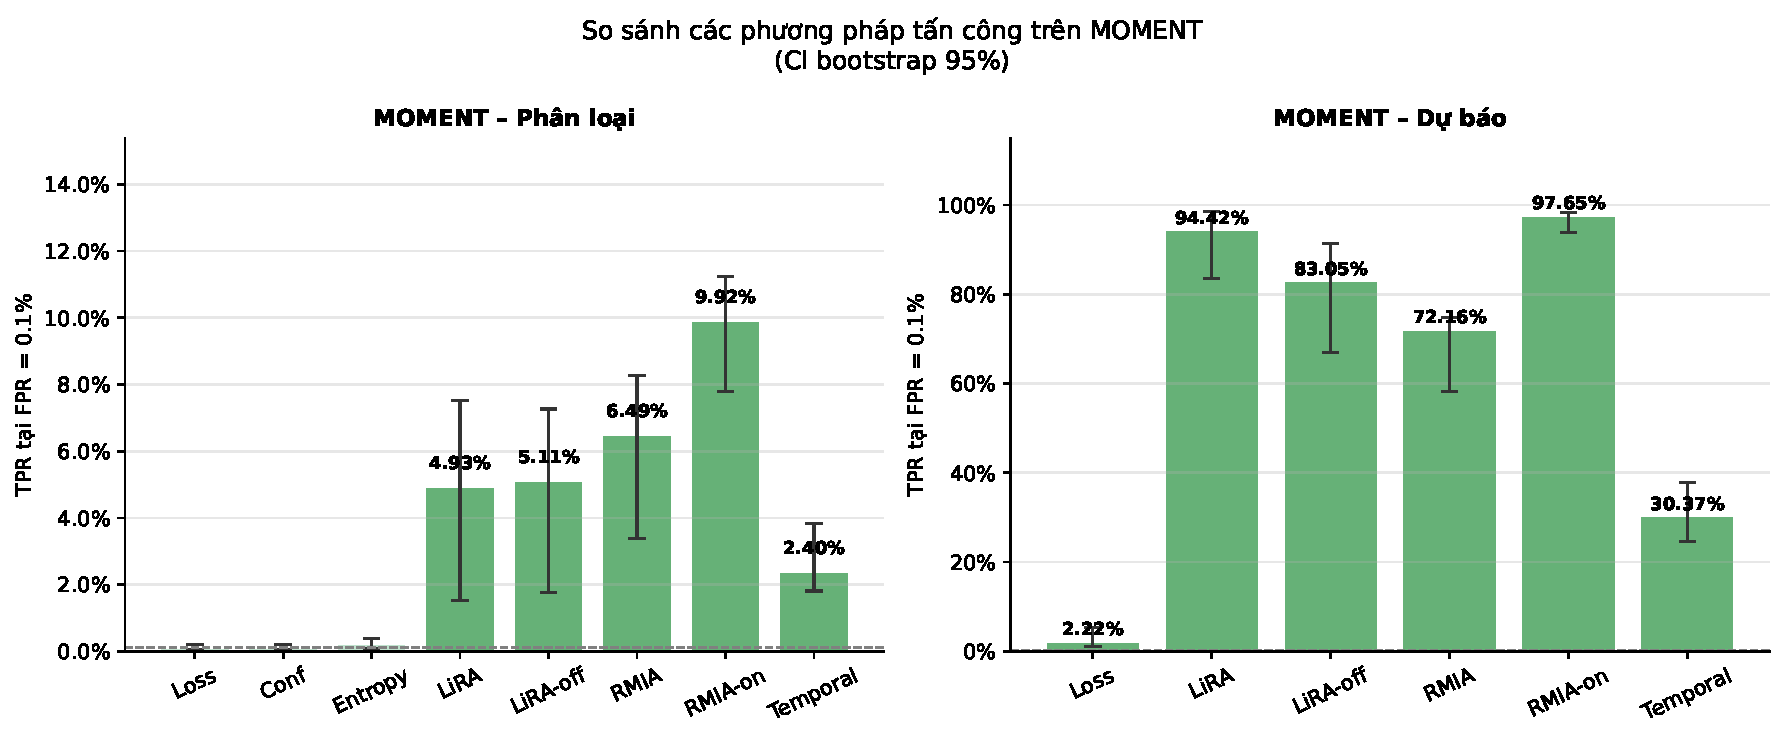
\includegraphics[width=\textwidth]{fig2_moment_attacks.pdf}
\caption{TPR@0,1\% FPR của các phương pháp tấn công trên MOMENT: phân loại (trái) và dự báo (phải). Lưu ý sự khác biệt lớn về trục y.}
\label{fig:moment_attacks}
\end{figure}

\textbf{Phân tích Bảng~\ref{tab:moment_fcst} và Hình~\ref{fig:moment_attacks}.} (1) Mọi tấn công dựa trên shadow gần như phân biệt hoàn hảo: RMIA-online $97{,}65\%$ (khoảng $7.945/8.136$ member bị nhận ra khi chỉ $\le 7$ non-member bị nhận nhầm; CI $[93{,}8\%; 98{,}3\%]$), LiRA $94{,}4\%$, LiRA-off $83{,}1\%$, RMIA $72{,}2\%$. (2) Biến thể offline, không cần biết bản ghi mục tiêu lúc huấn luyện shadow, vẫn đạt $72$--$83\%$, nên rủi ro không chỉ tồn tại ở giả định kẻ tấn công mạnh nhất. (3) Loss một mình chỉ $2{,}2\%$ ($22\times$ ngẫu nhiên) dù AUC $0{,}913$: nếu chỉ kiểm tra bằng Loss, người đánh giá sẽ đánh giá thấp rủi ro tới $\sim 44$ lần so với RMIA-online. (4) Temporal đạt $30{,}4\%$ (CI $[24{,}7\%; 37{,}8\%]$), cao gấp $\approx 12\times$ bộ phân loại chỉ dùng log-MSE ($2{,}5\%$): phổ và xu hướng của phần dư mang thông tin thành viên mà độ lớn sai số không có, tức MOMENT ghi nhớ \textit{hình dạng} dạng sóng của bản ghi huấn luyện, không chỉ giảm sai số. (5) Gap MSE $0{,}446$ ($\text{test}/\text{train} \approx 2{,}2\times$) là rất lớn, song iTransformer có gap tương đương ($0{,}477$) mà rò rỉ black-box thấp hơn hai bậc độ lớn; vì vậy gap là điều kiện cần nhưng không đủ, và tại sao MOMENT lại đặc biệt dễ bị tấn công vẫn là câu hỏi mở.

\section{Các hiện tượng bão hòa và suy biến điểm số}
\label{sec:artifacts}

Kiểm tra trực tiếp điểm số trong các tệp kết quả cho thấy hai trường hợp mà TPR hoặc AUC không phản ánh đúng sức mạnh tấn công:
\begin{itemize}
  \item \textbf{iTransformer, phân loại, Loss/Conf:} $97{,}2\%$ member có điểm bão hòa chính xác ($-\mathrm{CE} = 0$, hoặc xác suất $=1$), cùng với $22{,}3\%$ (Loss) và $32{,}0\%$ (Conf) non-member. Hệ quả: AUC $0{,}86$--$0{,}90$ nhưng TPR@1\% FPR $= 0$ (Mục~\ref{sec:itrans_analysis}).
  \item \textbf{TCN, dự báo, RMIA-online:} điểm của toàn bộ non-member bằng $0$ và member chỉ nhận $5$ giá trị khác nhau; chỉ khoảng $3{,}95\%$ member có điểm dương. Vì thế TPR@0,1\% $=$ TPR@1\% $= 0{,}0395$ và AUC $= 0{,}520$. Đây là sự bão hòa của phép đếm RMIA với $\gamma = 2$, không phải khả năng bảo vệ của TCN; bảng chỉ nên được đọc qua LiRA ($13{,}8\%$).
\end{itemize}
Cả hai trường hợp cho thấy việc báo cáo TPR cần đi kèm kiểm tra phân phối điểm số (tỉ lệ điểm trùng nhau tại giá trị cực trị).

\section{Bảng tóm tắt kết quả}

Bảng~\ref{tab:summary} liệt kê tấn công tốt nhất (theo TPR@0,1\% FPR, trong cả tám cấu hình). Bảng~\ref{tab:main_attacks} thu hẹp về các tấn công \textit{chính} theo protocol (loại LiRA-offline và RMIA-online) để so sánh công bằng giữa các mô hình.

\begin{table}[H]
\centering
\caption{Tóm tắt: tấn công tốt nhất (trong cả tám cấu hình) theo TPR@0,1\% FPR.}
\label{tab:summary}
\begin{tabular}{llcccc}
\toprule
\textbf{Mô hình} & \textbf{Bài toán} & \textbf{TPR@0,1\%} & \textbf{TPR@1\%} & \textbf{Tấn công tốt nhất} & \textbf{Dự báo/Phân loại} \\
\midrule
LSTM & Phân loại & 0,0061 & 0,0270 & LiRA-offline & -- \\
LSTM & Dự báo & 0,1309 & 0,4302 & RMIA-online & $21,3\times$ \\
TCN & Phân loại & 0,0817 & 0,1659 & RMIA-online & -- \\
TCN & Dự báo & 0,1383 & 0,3741 & LiRA & $1,7\times$ \\
PatchTST & Phân loại & 0,0184 & 0,0735 & RMIA-online & -- \\
PatchTST & Dự báo & 0,2848 & 0,5281 & RMIA-online & $15,4\times$ \\
iTransformer & Phân loại & 0,0773 & 0,2710 & Temporal & -- \\
iTransformer & Dự báo & 0,1400 & 0,4586 & Temporal & $1,8\times$ \\
MOMENT & Phân loại & 0,0992 & 0,1724 & RMIA-online & -- \\
MOMENT & Dự báo & \textbf{0,9765} & \textbf{0,9986} & RMIA-online & $9,8\times$ \\
\bottomrule
\end{tabular}
\end{table}

\begin{table}[H]
\centering
\caption{TPR@0,1\% FPR của các tấn công \textit{chính} theo protocol (``Đơn giản = giá trị lớn nhất trong Loss/Conf/Entropy; riêng dự báo chỉ có Loss). In đậm: tấn công chính tốt nhất mỗi dòng.}
\label{tab:main_attacks}
\begin{tabular}{llcccc}
\toprule
\textbf{Mô hình} & \textbf{Bài toán} & \textbf{Đơn giản} & \textbf{LiRA} & \textbf{RMIA (off)} & \textbf{Temporal} \\
\midrule
LSTM & Phân loại & 0,0017 & 0,0038 & \textbf{0,0045} & 0,0009 \\
TCN & Phân loại & 0,0007 & 0,0457 & \textbf{0,0520} & 0,0216 \\
PatchTST & Phân loại & 0,0021 & 0,0095 & \textbf{0,0136} & 0,0080 \\
iTransformer & Phân loại & 0,0057 & 0,0076 & 0,0127 & \textbf{0,0773} \\
MOMENT & Phân loại & 0,0022 & 0,0493 & \textbf{0,0649} & 0,0240 \\
\midrule
LSTM & Dự báo & 0,0182 & \textbf{0,0874} & 0,0600 & 0,0123 \\
TCN & Dự báo & 0,0044 & \textbf{0,1383} & 0,0176 & 0,0070 \\
PatchTST & Dự báo & 0,0079 & \textbf{0,1716} & 0,0873 & 0,0181 \\
iTransformer & Dự báo & 0,0299 & 0,0106 & 0,0116 & \textbf{0,1400} \\
MOMENT & Dự báo & 0,0222 & \textbf{0,9442} & 0,7216 & 0,3037 \\
\bottomrule
\end{tabular}
\end{table}

\textbf{Phân tích.} (1) Khi chỉ xét tấn công chính, kết luận định tính không đổi nhưng độ lớn giảm: MOMENT dự báo $94{,}4\%$ (LiRA), PatchTST dự báo $17{,}2\%$ thay vì $28{,}5\%$, và các tấn công RMIA-online ở Bảng~\ref{tab:summary} nên được xem là cận trên. (2) Tấn công thắng thay đổi theo mô hình và bài toán: LiRA/RMIA thắng ở 8/10 cấu hình, Temporal thắng ở cả hai bài toán của iTransformer; không có tấn công nào dominant, nên một kiểm toán quyền riêng tư nên chạy nhiều họ tấn công. (3) Cột ``Đơn giản'' hầu như luôn thấp nhất ở phân loại ($\le 0{,}57\%$), xác nhận Loss/Conf/Entropy gần ngẫu nhiên, nhưng ở dự báo Loss đạt $0{,}44$--$3{,}0\%$ (4--30 lần ngẫu nhiên), nên nhận định ``gần ngẫu nhiên'' chỉ đúng với phân loại.

% =============================================================
%  CHƯƠNG 7 – THẢO LUẬN
% =============================================================
\chapter{Thảo luận}
\label{chap:thaoluan}

\section{RQ1: Kiến trúc hiện đại vs.\ Baseline}

Trên phân loại, theo tấn công tốt nhất: LSTM ($0{,}61\%$) $<$ PatchTST ($1{,}84\%$) $<$ iTransformer ($7{,}73\%$) $\approx$ TCN ($8{,}17\%$) $\approx$ MOMENT ($9{,}92\%$), trong đó ba mô hình sau có CI chồng lấn. Trên dự báo: LSTM ($13{,}1\%$) $\approx$ TCN ($13{,}8\%$) $\approx$ iTransformer ($14{,}0\%$) $<$ PatchTST ($28{,}5\%$) $\ll$ MOMENT ($97{,}7\%$). Không có chiều hướng nhất quán ``kiến trúc hiện đại rò rỉ nhiều hơn/ít hơn baseline'': PatchTST rò rỉ nhiều hơn LSTM nhưng ít hơn TCN ở phân loại; iTransformer ngang TCN. Do đó RQ1 được trả lời là \textit{không có ưu thế hệ thống của kiến trúc}.

Về vai trò của generalization gap, bằng chứng chia hai nửa. Ở phân loại, thứ tự gap (LSTM $0{,}052$ $<$ PatchTST $0{,}133$ $<$ MOMENT $0{,}179$ $<$ TCN $0{,}213$) khớp thứ tự TPR của các tấn công chính (Bảng~\ref{tab:main_attacks}) với LSTM $<$ PatchTST $<$ \{MOMENT, TCN\} (hai mô hình cuối có TPR $6{,}5\%$ và $5{,}2\%$, CI chồng lấn), ủng hộ giả thuyết gap quyết định. Nhưng (i) iTransformer có gap lớn nhất ($0{,}480$) mà LiRA/RMIA chỉ $\approx 1\%$ (do utility suy biến và bão hòa điểm số), và (ii) ở dự báo TCN có gap nhỏ nhất ($0{,}080$) mà vẫn rò rỉ $13{,}8\%$, ngang LSTM (gap $0{,}250$). Kết luận thận trọng: gap là điều kiện cần cho tấn công điểm số đơn giản (Yeom et al.\ \cite{yeom2018}), nhưng tấn công hiệu chỉnh theo độ khó rò rỉ được ngay cả khi gap trung bình nhỏ. Lưu ý các mô hình không được so ở \textit{cùng} gap như RQ1 đặt ra; nhóm chọn epoch/lr theo utility trên tập val chứ không khớp gap.

\section{RQ2: Phân loại vs.\ Dự báo}

Trên cả năm mô hình, tấn công tốt nhất ở dự báo đạt TPR@0,1\% cao hơn phân loại, với hệ số $1{,}7\times$ (TCN), $1{,}8\times$ (iTransformer), $9{,}8\times$ (MOMENT), $15{,}4\times$ (PatchTST) và $21{,}3\times$ (LSTM); mức tăng tuyệt đối lần lượt $+5{,}7$, $+6{,}3$, $+87{,}7$, $+26{,}6$ và $+12{,}5$ điểm phần trăm. Với TCN và iTransformer, chênh lệch nhỏ và (với iTransformer) không có ý nghĩa thống kê (Hình~\ref{fig:cls_vs_fcst}).

Hai lý giải khả dĩ, cần đọc như giả thuyết: \textbf{(1) Tín hiệu dày đặc hơn.} Dự báo trả về $12 \times 96 = 1.152$ giá trị liên tục, mỗi giá trị là một phép đo ghi nhớ; phân loại chỉ trả về $5$ xác suất dễ bão hòa (iTransformer, TCN). Điểm $\phi = -\log\mathrm{MSE}$ là đại lượng liên tục, không bão hòa như $\log\frac{p}{1-p}$. \textbf{(2) Bản chất mục tiêu huấn luyện.} Hồi quy $L_2$ trên toàn bộ dạng sóng khuyến khích khớp chi tiết từng bản ghi, còn cross-entropy chỉ cần phân tách $5$ lớp. Chênh lệch $12{,}5$--$87{,}7$ điểm phần trăm vẫn có thể bị khuếch đại bởi số epoch dự báo (50) lớn hơn phân loại (20) ở LSTM, TCN và PatchTST. Phép so sánh không bị yếu tố này ở MOMENT (10/10 epoch) và iTransformer (50/50), cho kết quả $9{,}8\times$ và $1{,}8\times$. Lưu ý rằng gap của dự báo (MSE) và gap của phân loại (accuracy) có đơn vị khác nhau nên không thể so trực tiếp bằng số.

\section{Hàm ý bảo mật}

\begin{enumerate}
  \item \textbf{Không nên chỉ dùng tấn công đơn giản để kiểm tra quyền riêng tư.} Ở phân loại, Loss/Conf/Entropy gần ngẫu nhiên ở low-FPR trong khi LiRA/RMIA phát hiện được rò rỉ (TCN: $0{,}07\%$ so với $8{,}2\%$); ở dự báo MOMENT, Loss cho $2{,}2\%$ so với $97{,}7\%$. Một hệ thống chỉ kiểm bằng Loss có thể bị tuyên bố ``an toàn'' sai.
  \item \textbf{Cần kiểm tra phân phối điểm số và chạy nhiều họ tấn công.} Bão hòa (iTransformer) và suy biến (TCN RMIA-online) làm một tấn công đơn lẻ cho kết quả sai lệch; không có tấn công nào thắng ở mọi cấu hình.
  \item \textbf{Foundation model tinh chỉnh trên dữ liệu y tế cần đánh giá đặc biệt.} Với MOMENT dự báo, ở FPR $0{,}1\%$ (khoảng 1 trong 1.000 bản ghi non-member bị nhận nhầm) có tới $\approx 94$--$98\%$ bản ghi huấn luyện bị nhận diện đúng; với phân loại là $\approx 6$--$10\%$.
  \item \textbf{Mô hình dự báo có rủi ro cao hơn phân loại trên cùng dữ liệu,} nhất là khi tinh chỉnh mô hình lớn; cần cơ chế bảo vệ (differential privacy, perturbation đầu ra, giới hạn truy vấn, dừng huấn luyện sớm) và nên đo lại sau khi áp dụng.
\end{enumerate}

\section{Hạn chế}
\label{sec:limitations}

\begin{itemize}
  \item \textbf{Độ phân giải của low-FPR:} 7.636 non-member (dưới mục tiêu 10.000) cho phép khoảng 7 nhận nhầm ở FPR $0{,}1\%$; TPR@0,1\% nhiễu, CI rộng (tới $\pm 12$ điểm phần trăm ở LiRA-off của MOMENT dự báo). Chỉ bootstrap trên bản ghi đánh giá, không phản ánh phương sai do huấn luyện.
  \item \textbf{Một lần huấn luyện mỗi mô hình (seed $42$):} chưa có CI qua nhiều lần huấn luyện; các khác biệt nhỏ giữa mô hình (ví dụ TCN so với MOMENT ở phân loại) không kết luận được.
  \item \textbf{Chia record-level:} có ít nhất 266 bệnh nhân xuất hiện ở cả member và non-member; kết quả không áp dụng nguyên cho mức người dùng (Johansson et al.\ \cite{johansson2025} ghi nhận mức người dùng thường dễ tấn công hơn).
  \item \textbf{Công thức huấn luyện không đồng nhất:} epoch, learning rate, utility khác nhau giữa các mô hình; iTransformer phân loại gần như không tổng quát hóa (test $0{,}52$). RQ1 ``ở cùng gap'' không được thỏa.
  \item \textbf{Thiên lệch chọn tấn công tốt nhất} và $K = 8$ shadow model nhỏ; các biến thể online giả định kẻ tấn công biết bản ghi mục tiêu.
  \item \textbf{MOMENT:} chỉ full fine-tune, không có đối chứng; lịch sử theo epoch chỉ có tấn công Loss.
  \item \textbf{Temporal} là gray-box (cần nhãn member/non-member và checkpoint trung gian), không so ngang hàng với tấn công black-box.
  \item \textbf{Một tập dữ liệu} (PTB-XL) và chưa thử biện pháp phòng thủ.
\end{itemize}

% =============================================================
%  CHƯƠNG 8 – KẾT LUẬN
% =============================================================
\chapter{Kết luận}
\label{chap:ketluan}

Báo cáo đánh giá hệ thống tấn công suy luận tư cách thành viên trên năm mô hình chuỗi thời gian (LSTM, TCN, PatchTST, iTransformer, MOMENT) với tập ECG PTB-XL (seed $42$) theo tiêu chuẩn low-FPR. Nhóm rút ra các kết luận sau, kèm mức độ chắc chắn:

\begin{enumerate}
  \item \textbf{Dự báo rò rỉ nhiều hơn phân loại ở cả năm mô hình,} với mức tăng $1{,}7\times$ đến $21\times$ ($+5{,}7$ đến $+87{,}7$ điểm phần trăm). Kết luận chắc chắn với LSTM, PatchTST, MOMENT; yếu với TCN và iTransformer (hệ số $< 2\times$, iTransformer không có ý nghĩa thống kê).
  \item \textbf{MOMENT tinh chỉnh toàn bộ rò rỉ nhiều nhất,} đặc biệt ở dự báo ($97{,}7\%$ TPR tại $0{,}1\%$ FPR, tấn công chính $94{,}4\%$, AUC $\approx 1$). Ở phân loại mức rò rỉ ($9{,}9\%$) chỉ ngang TCN và iTransformer. Rò rỉ xuất hiện chủ yếu ở các epoch cuối.
  \item \textbf{Tấn công điểm số đơn giản không đủ.} Ở phân loại, Loss/Conf/Entropy gần ngẫu nhiên tại $0{,}1\%$ FPR; ở dự báo Loss thấp hơn LiRA/RMIA tốt nhất từ $7$ đến $44$ lần (trừ iTransformer, nơi Loss lại cao hơn LiRA). Không tấn công nào thắng ở mọi cấu hình (LiRA/RMIA thắng 8/10, Temporal thắng với iTransformer), và bão hòa/suy biến điểm số có thể làm sai lệch một tấn công đơn lẻ.
  \item \textbf{Kiến trúc hiện đại không rò rỉ hệ thống hơn hay ít hơn baseline;} generalization gap giải thích tốt thứ tự ở phân loại nhưng không giải thích được iTransformer hay TCN dự báo.
\end{enumerate}

Hướng tiếp theo: (i) huấn luyện lặp nhiều seed và mở rộng non-member lên $\ge 10.000$; (ii) đối chứng cho MOMENT (huấn luyện từ đầu, encoder đóng băng, đánh giá theo epoch cho tấn công shadow); (iii) chia theo bệnh nhân (user-level); (iv) thêm UCI HAR và ETTh1; (v) đánh giá differential privacy (DP-SGD) và các biện pháp phòng thủ khác.


% =============================================================
%  TÀI LIỆU THAM KHẢO
% =============================================================
\bibliographystyle{IEEEtran}
\bibliography{references}

\end{document}
